% 这是有限群附录

\chapter{Finit Group}
\epigraphhead[40]{\epigraph{数学书有两种,一种是看一面就看不下去的,一种是看了一行就看不下去的。}{杨振宁}}
这篇附录是根据李新征老师群论讲义和教学录像整理而成的笔记, 大致只打算写完有限群, 对于高量学习绰绰有余。
\section{群的基本结构}
\subsection{群的定义和一些基本定理}
其实在接受前面对于线性空间的抽象定义之后也很好接受群的概念:
\begin{define}{群的定义}
    群是一个有着\textbf{乘法}$\circ$这一特殊结构的元素集合$G$:
    \begin{itemize}
    \item[$\bullet$] \textbf{封闭性}:$\forall g_1,g_2\in G\rightarrow g_1\circ g_2\in G$
    \item[$\bullet$] \textbf{结合律}:$(g_1\circ g_2)\circ g_3=g_1\circ (g_2\circ g_3)$
    \item[$\bullet$] \textbf{单位元(幺元)存在性}:$\exists e\in G,\mathrm{s.t.}\forall g\in G\rightarrow g\circ e=e\circ g=g$
    \item[$\bullet$] \textbf{逆元存在性}:$\forall g\in G,\exists g^{-1}\in G\rightarrow g\circ g^{-1}=g^{-1}\circ g=e$
    \end{itemize}
\end{define}
上面的定义中不必额外强调单位元和逆元的唯一性, 因为根据定义唯一性自动存在。而且有\footnote{后面在不引起歧义时, 省略乘法符号}:
\begin{equation*}
    (g_1g_2)^{-1}=g_2^{-1}g_1^{-1}
\end{equation*}

不过要注意, 一般的群的乘法是\textbf{不满足}交换律的, \textbf{乘法额外满足交换律的群我们称之为Abel群}。
\begin{example}{群的例子}
    全体整数$\mathbb{Z}$在自然加法作为乘法的情况下构成一个群, 而且还是一个Abel群。
\end{example}
\begin{define}{群的阶}
    群的阶的定义和集合的势的概念是相通的, 定义为群内元素的个数, 记为$|G|$, 常说的有限群指的就是群的阶有限大。
\end{define}
下面要介绍的定理是后面的证明几乎都需要用到的定理:
\begin{theorem}{重排定理}
    \begin{equation*}
        gG=Gg=G
    \end{equation*}
    其中$g\in G$, 其实就是说$G$中拿出一个元素再去和$G$中的所有元素相乘, 得到的集合还是原来的群$G$本身, 而且不会出现重复。$g$的作用只是把原先的群元素重新排列了一下。
\end{theorem}
\begin{proof}
     $(1)\forall g_\alpha \in G$,由逆元存在性和封闭性知$g^{-1}g_\alpha \in G$,那么再根据结合律和逆元定义知$g(g^{-1}g_\alpha)=g_\alpha$,那么当
    $g_\alpha$取遍$G$中元素我们便得到了$gG=G$.\\
    $(2)$用到群相关定理证明的大杀器:{\color{red}{反证法}},设$g_\alpha\neq g_\beta$,如果$gg_\alpha=gg_\beta$,那么$g^{-1}(gg_\alpha)=g^{-1}(gg_\beta)\Rightarrow g_\alpha= g_\beta$,
    与已知矛盾.这一证明其实用掉了群的所有性质.\qed
\end{proof}
\subsection{群的内部结构}
\begin{define}{子群}
    设$H$是群$G$的一个子集, 如果$H$中的元素在$G$的乘法定义下也构成一个群, 那么就称$H$是$G$的一个子群, 记为$H\leq G$
\end{define}
\begin{example}{平庸子群}
    显然任何群$G$的幺元和其本身是$G$的两个子群,我们称之为平庸子群,其它的我们称为$G$的固有子群。
\end{example}
\begin{define}{循环子群和群元的阶}
    对任意一个\textbf{有限群}$G$,从中任取一个元素$a$,在原先的群乘法定义下作幂操作,\uwave{总是}可以得到一个$G$的子群$Z_k\equiv{a,a^2,a^3,\ldots,a^k=e}$,我们称之为
    $G$的一个循环子群,这个子群的阶,或者说使得$a^k=e$的最小的$k$称之为群元$a$的阶.
\end{define}
这里需要额外说明的就是为啥任何一个元素一定可以生成一个循环子群。只需要说明使$a^k=e$的$k$一定存在,$a=e$,问题解决;$a\neq e$,那么$a^2\neq a$否则$a=e$,$a^2=e$那么问题解决,
但如果$a^2\neq e$,就再考虑$a^3$,如此下去,由于前提是$G$为有限群,所以这个$k$一定存在。
\begin{define}{陪集}
    设$H\leq G$,由固定的$g\in G$可以生成$H$的左陪集:$gH\equiv{gh|h\in H}$,或是右陪集:$Hg\equiv{hg|h\in H}$
\end{define}
注意上面的定义中我们并没有用“群”这个字眼,说明陪集这个玩意一般只是一个集合而已,没有群结构。不难证明陪集中的元素是和子集$H$中的元素一一对应的,根据重排定理,
$g\in H$时$gH$和$Hg$构成一个群,就是$H$本身。
\begin{theorem}{陪集定理}
    $H\leq G, g_1,g_2\in G\rightarrow \{g_1H=g_2H\}\oplus \{g_1H \cap g_2H=\varnothing\}$\footnote[0]{其中$\oplus$表示“异或”,表示两者只能取其一。}
\end{theorem}
这个定理使用重排定理和反证法很好证明,只需要说明只要两个左陪集有一个公共元素那么$g_1H=g_2H$即可。当然,这个定理对于右陪集一样适用。这个定理也告诉我们或许任意一个群可以分解为一系列其某个子群的陪集的不交并。
\begin{proposition}{陪集分解}
    $H\leq G$,则$G$一定可以分解为一系列陪集的不交并,及:
    \begin{equation*}
        G=eH+g_1H+g_2H+\cdots
    \end{equation*}
\end{proposition}
根据前面的陪集定理,我们只需要在构建这个分解时,不断选取$g_\alpha$不属于前面的集合去构建新的陪集$g_\alpha H$即可。前面我们说过陪集元素和$H$一一对应,那么$|gH|=|H|$,再看陪集分解,由
于我们可以将任意一个集合分解为一系列陪集的\textbf{不交并},所以我们立即得到下面的Lagange定理:
\begin{theorem}{Lagrange定理}
    有限子群的阶必为群的阶的因子,也就是说$|H|$一定可以整除$|G|$
\end{theorem}
\begin{define}{共轭}
    $\forall f,h\in G$,如果$\exists g\in G$,使得$gfg^{-1}=h$,我们就称这两个元素共轭,记为$f\sim h$
\end{define}
群元素共轭的概念抽象一点这就是集合中的\textbf{等价关系的概念},满足下面三条:
\begin{itemize}
    \item[$\bullet$] \textbf{对称性}:$f\sim h\rightarrow h\sim f$
    \item[$\bullet$] \textbf{传递性}:$f_1\sim h,h\sim f_2\rightarrow f_1\sim f_2$
    \item[$\bullet$] \textbf{反身性}:$f\sim f$
\end{itemize}
上面的三条性质共轭全部满足,说的具体一点所有的$n\times n$矩阵构成一个群(这其实是个无限群),共轭的概念就是矩阵之间的相似概念。
\begin{define}{类}
    群$G$可按共轭关系分割成一些等价类$A_a={gag^{-1}|\forall g\in G}$.称$A_a$为群$G$的元素$a$的共轭类,简称为群的$a$类.
\end{define}
共轭类有下面的性质:
\begin{itemize}
    \item (1)单位元素$e$自称一类;
    \item (2)Abel群中的所有元素都自成一类;
    \item (3)类中的所有元素的阶都相等。
\end{itemize}

由于两个共轭类之间也有类似陪集之间的不相交的性质,所以我们也很容易实现将一个群用其群元的类来分解,只要对每个元素确定其类即可。不过前面的陪集分解是分解为一系列
大小相等的等份,而按照类的分解就不一定是等分了,不过还是有下面类似的定理:
\begin{theorem}{类中的元素个数}
    有限群的每个元素确定的类中的元素的个数都是群的阶的因子
\end{theorem}
\begin{proof}
    我们的目的是找到群的任意元素$g$确定的类的元素个数。

    证明这个定理的第一步是证明$\forall g\in G$,定义$H_g\equiv\{h\in G|gh=hg\}$,也就是所有与$G$中元素互易的元素构成了$G$的一个子群。由于子群乘法的定义来源于$G$,是良好定义的,
    所以我们只需要证明封闭性和逆元存在性。

    先证封闭:$gh_1=h_1g,gh_2=h_2g\rightarrow gh_1h_2=h_1gh_2=h_1h_2g$

    再证有逆:$gh=hg\rightarrow h^{-1}g^{-1}=g^{-1}h^{-1}\rightarrow gh^{-1}=h^{-1}g\rightarrow h^{-1}\in H_g$

    第二步是将$G$陪集分解为$\{g_0H_g,g_1H_g,\ldots\}$,其中$g_0$是幺元。注意到每个陪集$g_iH_g$中,$h_\alpha$取遍$H_g$,也就是$g_i h_\alpha$取遍$g_iH_g$中的所有元素时,
    $(g_i h_\alpha )g(g_i h_\alpha )^{-1}$给出的是和$g$共轭的元素这是毋庸置疑的,我们要是能进一步证明其实给出的还是同一个元素,我们记为$\tilde{g_i}$,我们就把陪集$g_iH_g$和$g$类中的元素
    对应起来了,如果不同的陪集给出不同的元素,也就说还可证明这种对应是一一对应的。那么根据Lagrange定理,陪集$g_ih_g$将$G$等分,而$g$类中元素个数就是等分的份数,也就是$|G|$的因子。下面着手证明:

    $(1)$一个陪集对应一个$g$类中元素:$(g_i h_\alpha )g(g_i h_\alpha )^{-1}=(g_i h_\alpha )g( h_\alpha^{-1}g_i^{-1} )=g_i (h_\alpha g) h_\alpha^{-1}g_i^{-1}
    =g_i  g(h_\alpha h_\alpha^{-1})g_i^{-1} =\tilde{g_i}$
    
    $(2)$不同陪集给出不同元素:假设$g_iH_g\neq g_j H_g$,那么如果对应的元素相等:$g_igg_i^{-1}=g_jgg_j^{-1}$,那么$(g_j^{-1}g_i)g=g(g_j^{-1}g_i)\rightarrow g_j^{-1}g_i\in H_g$,
    根据重排定理$g_j^{-1}g_iH_g=H_g\rightarrow g_iH_g=g_jH_g$,与假设矛盾。\qed
\end{proof}
\begin{define}{共轭子群}
    $H\leq G,K\leq G$,如果$\exists g\in G\rightarrow gHg^-1\equiv\{ghg^{-1}|h\in H\}=K$
\end{define}
这个定义完全是照搬群元共轭的,后面用到的机会也不多。
\begin{define}{正规子群(不变子群)}
    如果子群$H$中的所有元素的同类元素都属于$H$,那么称$H$是$G$的不变子群或者说正规子群,在群元共轭操作下是不变的,记为$H\unlhd G$.
\end{define}
下面这个定理是和前面的定义等价的,有的书常常也用这个定理作为正规子群定义。
\begin{theorem}{正规子群左右陪集完全重合}
    $H\unlhd G\iff \forall g\in G,gH=Hg$
\end{theorem}
\begin{proof}
    先证必要性,等价于证明$H\unlhd G\rightarrow gHg^{-1}=H$.

    根据正规子群的定义,$\forall h_\alpha\in H\rightarrow gh_\alpha g^{-1}\in H\rightarrow gHg^{-1}\subseteq H$,反过来,还是根据正规子群的定义以及$g^{-1}\in G$,
    $\forall h_\alpha\in H$,一定存在$h_\beta\in H$,使得$g^{-1}h_\alpha (g^{-1})^{-1}=h_\beta$成立,而这意味着$h_\alpha=g h_\beta g^{-1}\in gHg^{-1}$,也就是说$gHg^{-1}\supseteq H$.这样我们便证明了必要性.

    再证充分性,$\forall h_\alpha\in H$,根据左右陪集相等,一定存在$h_\beta\in H$,使得$gh_\alpha g^{-1}=h_\beta$,而$g$是在$G$中任取的,这也便直接说明了$H$中元素的类都属于$H$.
    \qed
\end{proof}
对于正规子群,今后不用再区分左右陪集。
\begin{theorem}{两个陪集中元素的乘积必为第三个陪集中的元素}
    $H\unlhd G$,取$g_1H\neq g_2H$,且两陪集都不是子群本身,那么$\forall g_1h_\alpha\in g_1H,g_2h_\beta\in g_2H\rightarrow g_1h_\alpha g_2h_\beta\in g_3H$,其中$g_3H\neq g_1H,g_3H\neq g_2H$
\end{theorem}
\begin{proof}
    如果$g_1H=g_2H=g_0H$,两个陪集都是子群本身,那么显然得到的元素都是$H$中的元素;

    如果$g_1H,g_2H$中有一个是$g_0H$,那么显然最后得到的元素要么是$g_1H$中元素,要么是$g_2H$中元素。

    现在考虑$g_1H$和$g_2H$都不是$H$的情况,$g_1h_\alpha g_2 h_\beta=g_1g_2(g_2^{-1}h_\alpha g_2 )h_\beta$,根据正规子群定义,$g_2^{-1}h_\alpha g_2\equiv h_{\alpha^\prime}\in H$,
    如果$g_1h_{\alpha} g_2 h_\beta\in g_1H$,那么$\exists h_\gamma\in H$,使得$g_1h_\gamma=g_1g_2h_{\alpha^\prime} h_\beta\rightarrow g_2=h_\gamma h_\beta^{-1} h_{\alpha^\prime}^{-1}\in H$,根据重排定理这直接说明$g_2 H=H$.与假设矛盾,关于$g_1$的情形是对称的
    ,证明略去. 

    而且这个证明还让我们了解到这个新的陪集是$g_1g_2H$,所以两个陪集中的元素相乘给出的新的元素都来自于同一个新的陪集。
    
    你还可以简单的接纳下面这个非常\uwave{物理仁}的证明:\[(g_1H)(g_2H)=g_1(Hg_2)H=g_1(g_2H)H=g_1g_2(HH)=g_1g_2H\]
    
    \qed
\end{proof}
\begin{define}{商群}
    $H\unlhd G$,用这个不变子群对$G$进行陪集分解:$\{g_0H,g_1H,g_2H,\ldots,g_nH\}$.把其中的每一个陪集当作是一个新的元素,记$f_i=g_iH$.
    对这个陪集的集合定义新的乘法,$f_if_j=f_k$表示陪集$g_iH$和$g_jH$中的元素相乘得到$g_kH$中的元素.\textbf{那么这个陪集的集合在这个乘法的定义下构成一个群,称作$G$的一个商群},记为$G/H$.
\end{define}
这个概念其实有点像线性空间里面的仿射子集建立的商空间。
\subsection{同构与同态}
\begin{define}{群同构}
    若从群$G\circ$到$F\star$上\footnote{后面的符号表示群乘法符号}存在一个一一对应的映射(同时满足单性和满性)$\Phi:G\mapsto F$,而且满足\textbf{乘积的映射等于映射的乘积}:
    \begin{equation}
        \label{eq:D.1}
        \Phi(g_1\circ g_1)=\Phi(g_1)\star\Phi(g_2),\forall g_1,g_2\in G
    \end{equation}
    那么我们就称群$G$和$F$是同构的,记作$G\cong F$.
\end{define}
其实群的同构意味着两个群实质上代数结构完全一致,只是看起来指代不同的内容,关系过强从而意义有时并不大,下面我们弱化一下刚才的定义,得到所谓群同态的定义。
\begin{define}{群同态}
    若$\exists \Phi:G\mapsto F$,这个映射可以是多对一的,也不必是满映射,但是仍满足乘积的映射等于映射的乘积(\ref{eq:D.1}). 我们便称$G$与$F$同态,记为$G\sim F$.
\end{define}
上面的定义是数学中的定义,但物理中用的比较多的同态关系满足$\Phi(G)=F$,也就是说$\Phi$是满映射,这样我们之后表述定理就不必像数学家那样去用$\mathrm{range}\Phi$表述了,所以
之后谈同态,{\color{red}默认$\Phi$是满映射}。
\begin{figure}[h]
    \centering
    \subfigure[同构关系]{
        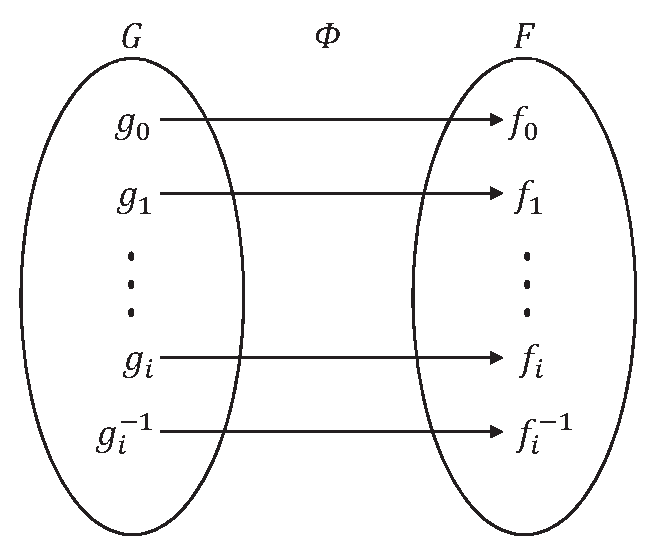
\includegraphics[width=0.4\linewidth]{fig/fig_D.1a.eps}
    }
    \quad
    \subfigure[同态关系]{
        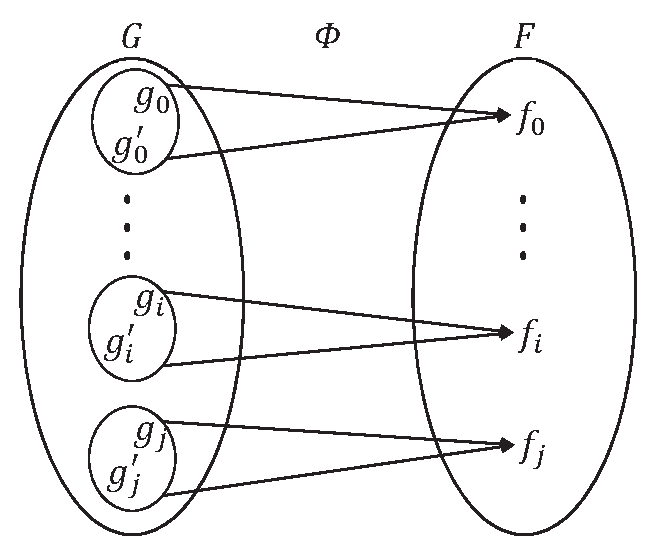
\includegraphics[width=0.4\linewidth]{fig/fig_D.1b.eps}
    }
    \caption{同构与同态}
    \label{fig:D.1}
\end{figure}
我们还可以很容易得到同态和同构映射的两个重要性质:
\begin{itemize}
    \item \textbf{幺元映射为幺元}:$\Phi(g_0)=f_0$
    \item \textbf{逆元映射为逆元}:$\Phi(g^{-1})=\Phi(g)^{-1}$
\end{itemize}
\begin{define}{同态核}
    $G$中所有与$F$中单位元素$f_0$所对应的元素的集合:
    \[\mathrm{Ker}\Phi\equiv\{h\in G|\Phi(h)=f_0\}\]
\end{define}
这个定义和线性代数里面线性映射的核(Kernel)\footnote{有的书也叫做零空间}的定义是类似的。
\begin{theorem}{同态核定理}
    设$G\cong F$,$H$是同态核,那么:
    \begin{itemize}
        \item $H\unlhd G$
        \item $G/H\cong F$
    \end{itemize}
    注意这个定理的表述默认$\Phi$是满的,否则要用$\mathrm{Im}\Phi$替换$F$
\end{theorem}
\begin{proof}
    第一点是比较容易证明的,首先不难$H$是子群,我们再稍微说明一下它是不变子群。我们要证明的实际上是$\forall h\in H,\forall g\in G\rightarrow ghg^{-1}\in H$,注意到
    $\Phi(ghg^{-1})=\Phi(g)\Phi(h)\Phi(g^{-1})=\Phi(g)\Phi(g^{-1})=f_0$,便直接证明$H\unlhd G$.

    第二点的证明我们实际上是需要去构建一个合适的同构映射,我们自然的可以想到这样的一个映射,将$G/H$中的元素$g_iH$映射到$\Phi(g_i)$上,你可以按照前面的图\ref{fig:D.1}理解为图b中的每一个小圈圈对应$G/H$中的一个
    陪集,构造的同构映射就是在同态映射的基础上将每个小圈圈对应$F$中的一个元素. 根据同态的性质,满性已然成立,下面要证明的是单性,也就是不同陪集对应不同元素.

    还是利用反证法来证明. 设$g_iH$和$g_jH$是两个不同的陪集,但是对应相同的$F$中元素$f$,那么$\forall h\in H, \Phi(g_i^{-1}g_jh)=f^{-1}ff_0=f_0\rightarrow g_i^{-1}g_jh\in H\rightarrow g_i^{-1}g_j\in H$,
    再根据重排定理,$g_i^{-1}g_jH=H\rightarrow g_iH=g_jH$,与假设矛盾.
    \qed
\end{proof}

看前面的图\ref{fig:D.1},这个定理实际上是在说与$F$中单位元素$f_0$对应的子群是$G$的一个不变子群,其它的小圈圈是他的陪集,所以每个小圈圈中的元素个数都相等,而且把这些小圈圈
单独看成一个个元素构成的商群和$F$同构。

\begin{define}{自然同态}
    如果$K\unlhd G$,那么映射$\pi:G\mapsto G/K$将$g$映射为陪集$gK$,建立了$G$和$G/K$之间的一个满同态\footnote[1]{也就是说$\mathrm{range}\pi=G/K$},而且同态核为
    $\mathrm{Ker}\pi=K$.我们称这个同态映射$\pi$为群$G$的自然同态.
\end{define}
这个实际上进一步告诉我们同态核和正规子群是一样的,也就是说一个正规子群可以看做某个群同态的同态核,反之同态核一定是某个正规子群。证明的话其实就是同态核定理逆推回去。
\begin{define}{自同构映射}
    自同构映射建立的是群和它自己的同构映射,$\nu :G\mapsto G$,最平凡的例子就是恒等映射。    
\end{define}
\begin{define}{自同构映射群}
    所有的自同构映射构成了一个群,乘法定义就是复合映射概念,我们记为$A(G)$.
\end{define}
\begin{define}{内自同构映射}
    还有一类同构映射比较特殊,$\forall u\in G$,我们可以依此构造一个自同构映射,我们定义映射为$\nu(g)=ugu^{-1}$,其实就是去找某个与$g$同类的元素。和上面类似的,自同构映射放在一起也构成了一个群,
    即自同构映射群,记为$I(G)$.
\end{define}
下面我们证明\textbf{内自同构映射群是自同构映射群的不变子群}。
\begin{proof}
    $I(G)\leq A(G)$这一点很容易证明,下面我们要证明$\forall \mu\in I(G),\nu\in A(G)\rightarrow\nu\mu\nu^{-1}\in I(G)$. 设$g_\alpha,g_\beta\in G, 
    \mu(g_\alpha)=u g_\alpha u^{-1},\nu(g_\alpha)=g_\beta$,那么$\nu\mu\nu^{-1}(g_\beta)=\nu\mu(g_\alpha)=\nu(ug_\alpha u^{-1})=\nu(u)g_\beta \nu(u)^{-1}$,
    根据$I(G)$的定义便得知$I(G)\unlhd A(G)$.
    \qed
\end{proof}
\subsection{群作用与变换群}
\begin{define}{左右作用与伴随作用}
    $\bigstar$左作用:$\forall g\in G$可以定义一个左作用$L_g:G\rightarrow G$,效果为$\forall g^\prime \in G,L_gg^\prime\equiv gg^\prime$.
    
    $\bigstar$右作用:$\forall g\in G$可以定义一个右作用$R_g:G\rightarrow G$,效果为$\forall g^\prime \in G,R_gg^\prime\equiv g^\prime g^{-1}$.

    $\bigstar$伴随作用:$\forall g\in G$可以定义一个伴随作用$\mathrm{Ad}_g:G\rightarrow G$,效果为$\forall g^\prime \in G,\mathrm{Ad}_gg^\prime\equiv gg^\prime g^{-1}$.
\end{define}
伴随作用就是前面说的内自同构映射的概念,也是三个作用里面最为重要的一个,而其它两个都不是同构映射。

\begin{define}{变换和变换群}
    设变换对象$X$是一个非空集合,则双射$f:X\rightarrow X$称为$X$上的一个变换或置换。定义这些置换的乘法为$f\circ g(x)=f(g(x))$,则所有的这些置换构成了一个群,
    称为$X$上的完全对称群$S_X$, 一般所说的变换群是$S_X$的子群。如果$X$有$n$个元素,则称其上的完全对称群为$X$上的$n$阶置换群$S_n$.如果我们变换的对象还构成一个群,
    它也有完全对称群$S_G$.
\end{define}

回到前面左右作用的定义,我们发现右作用不是直接右乘,而是右乘逆元。$\forall g\in G$,我们可以确定左右作用$L_g,R_g$,而这个确定给每个群元确定一个左(右)作用的过程其实就是一个$G\to S_G$的映射,当然这个映射不是满的,
但是却是个同态映射,很容易确定$L_{gg^\prime}=L_gL_{g^\prime}$,$R$同理。
\begin{theorem}{Cayley定理}
    群$G$同构于其完全变换群$S_G$的一个子群
\end{theorem}
\begin{proof}
    显然$G$中生成的左作用$L_g$构成的群$\{L_g|g\in G\}$就是这个子群而且与$G$同构.\qed
\end{proof}
\begin{define}{等价与轨道}
    设$G$为$X$上的变换群,若对$x,y\in X,\exists g\in G$,使得$g(x)=y$,那我们便称$x$与$y$等价,记为$x\sim y$. $X$中所有与$x$等价的元素的集合称为$x$的$G$轨道:
    $\mathcal{O}_x^G\equiv\{g(x)|g\in G\}$.
\end{define}
\begin{define}{不变子集}
    设$G$为$X$上的变换群,$Y\subseteq X$,满足$G$中的任意元素$g$作用在$Y$中元素上得到的结果还属于$Y$,那我们称$Y$为群$G$在$X$上的不变子集。
\end{define}
其实这个概念和线性代数里面的不变子空间概念是很像的。$\mathcal{O}_x^G$以及它们的并显然就是一些不变子集。
\begin{define}{迷向子群}
    设$G$为$X$上的变换群,$x\in X$,若$G^{x}\leq G$且保持$x$不变,即$G^{x}=\{h\in G|h(x)=x\}$,则称$G^{x}$是$G$对$x$的迷向子群。
\end{define}
\begin{define}{$\mathcal{O}_x^G$和$G^{x}$的左陪集一一对应}
    $G^{x}$的每个左陪集把$x$映为其$G$轨道上的点,且不同陪集映射到不同点。
\end{define}
由此我们便知$|\mathcal{O}_x^G|=|G|/|G^{x}|$.
\subsection{直积与半直积}
笛卡尔直积$\times$的概念就是两个集合中各取一个元素构成一个有序对来生成新的集合,我们进一步定义这个集合元素间的乘法是可以将其升级为群的。
\begin{define}{直积群}
    两个群中各取一个群元$g_{1\alpha},g_{2\beta}$构成一个有序对$g_{\alpha\beta}=(g_{1\alpha},g_{2\beta})$,且定义乘法,$g_{\alpha\beta}\times g_{\alpha^\prime\beta^\prime}
    =(g_{1\alpha}g_{1\alpha^\prime},g_{2\beta}g_{2\beta^\prime})$. 在这个乘法意义下这些有序对形成了一个新的群$G$,记为$G_1,G_2$的直积群$G_1\otimes G_2$.
\end{define}
\begin{define}{直积分解}
    若群$G$中的元素都可以唯一地拆写为$g_{\alpha\beta}=g_{1\alpha}g_{2\beta}$,其中$g_{1\alpha}\in G_1,g_{2\beta}\in G_2$,而且两个群之间的元素乘法满足交换律,即$\forall g_1\in G_1,g_2\in G_2\rightarrow g_1g_2=g_2g_1$,那
    自然的我们便将$G$中元素写成了有序对的形式,而且$G=G_1\otimes G_2$,$G_1,G_2$称为直积因子。
\end{define}
\begin{theorem}{直积因子的结构关系}
    群$G$的直积因子$G_1$和$G_2$满足:
    \begin{itemize}
        \item \textbf{只有一个公共元素幺元}:$G_1\cap G_2={e}$
        \item \textbf{都是正规子群}:$G_1\unlhd G, G_2\unlhd G$
    \end{itemize}
\end{theorem}
\begin{proof}
    第一点使用反证法证明,如果$G_1\cap G_2=a\neq e$,那么$G$中元素$a$可以写为$a=a\cdot e=e\cdot a$,都是前者属于$G_1$后者属于$G_2$,但显然拆分不唯一,不是直和分解定义。

    再看第二点,以$G_1$为例。$\forall g_1\in G,g=g_\alpha g_\beta\in G\rightarrow (g_\alpha g_\beta)g_1(g_\alpha g_\beta)^{-1}=g_{\alpha} g_1 g_{\alpha}^{-1}\in G_1$\qed
\end{proof}

\begin{define}{半直积}
    对于群$G_1$,如果$G_2\sim A(G_1)$,也就是说对于$G_2$中任意一个元素都能找到对应的一个$G_1$群的自同构映射$\nu_{g_{2\beta}}$.我们定义$G_1$和$G_2$之间元素构成的有序对集合$G=\{\left \langle g_{1\alpha},g_{2\beta}\right\rangle\}$
    之间的乘法满足
    \[\left\langle {{g_{1\alpha }},{g_{2\beta }}} \right\rangle  \times \left\langle {{g_{1\alpha '}},{g_{2\beta '}}} \right\rangle  = \left\langle {{g_{1\alpha }}{\nu _{{g_{2\beta }}}}({g_{1\alpha '}}),{g_{2\beta }}{g_{2\beta '}}} \right\rangle \]
    这样构造的新群称为$G_1,G_2$的半直积群,记为$G_1 \rtimes G_2$.
\end{define}
要证明这样定义乘法的正确性,注意$\nu_{g_{\beta}}(g_{\alpha}g_{\alpha^\prime})=\nu_{g_{\beta}}(g_{\alpha})\nu_{g_{\beta}}(g_{\alpha^\prime})$和$\nu_{g_\alpha g_\beta}=\nu_{g\alpha}\nu_{g_\beta}$即可。

从定义就可以看出来$G_1,G_2$的地位不是对称的,实际上这里$G_1\unlhd G$而$G_2$不再有这一性质。

\section{群表示论}
这一节我们的首要任务就是将一个抽象的群用具体的矩阵表示出来,基本工具是附录B中的线性代数。
\subsection{群表示基本概念}
\begin{define}{线性变换群}
    定义线性空间$V$上两个线性变换的乘法为它俩的相继作用,那么$n$维复线性空间$V$上的全部\textbf{非奇异}线性变换构成了一个群,称为复一般线性变换群,记为$GL(V,\mathbb{C})$.
    用的更多的是它的任一子群$L(V,\mathbb{C})$称为$V$上的线性变换群。
\end{define}
上面的定义中需要注意的是\uwave{非奇异}这个条件,否则就不满足逆元存在这一条件了。另外,对于实向量空间,也可对应定义$GL(V,\mathbb{R})$、$L(V,\mathbb{R})$,只是用的少些罢了。

\begin{define}{线性表示}
    对于群$G$,如果存在一个从$G$到线性空间$V$上的某个线性变换群$L(V,\mathbb{C})$的同态映射$\mathscr{A}$,那么我们称$\mathscr{A}$是群$G$的一个线性表示,$V$是表示空间,
    $\dim V$是表示的维数。如果我们选取了$V$上的一组基,那么$\mathscr{A}(g)$就可以和一个矩阵$\mathcal{A}(g)$联系起来\footnote[1]{今后用花体$\mathscr{A}$作为群表示符号,手写体$\mathcal{A}$作为对应矩阵的符号。},所以物理上常常也就说群表示就是用矩阵表示一个抽象群。
\end{define}
\begin{define}{忠实表示}
    如果表示$\mathscr{A}$是一个同构映射,那我们称他为忠实表示。
\end{define}
从上面的这些定义可以看出群表示有无穷多个,比如把所有群元对应到恒等映射$\{I\}$就是一个表示,称为平庸表示,而且不同表示之间其实还可以相互联系,我们真正关系的是那些不可约且相互不等价的表示。
\begin{define}{等价表示}
    如果两个$V$上的表示$\mathscr{A},\mathscr{B}$可以由$V$上的一个非奇异变换$P$联系起来,即$\mathscr{B}(g)=P^{-1}\mathscr{A}(g)P$,其中$P$与群元$g$无关,我们就称
    两个表示等价。
\end{define}
这个还可以这么理解,我们在同一个基底下写下两个表示的矩阵$\mathcal{A},\mathcal{B}$,根据上面的定义,$\mathcal{B}=P^{-1}\mathcal{A}P$,也就是说这两组矩阵由一个相似变换联系起来,
况且我们还知道,两个相似的矩阵可以看成是同一个线性变换在不同基底下的矩阵表示,基于这些,我们便可以理解为啥这么定义表示等价了。

等价表示还可以稍微推广一下,$\mathscr{A}$和$\mathscr{B}$不一定要是同一个表示空间,若它们处于两个同维的(也必定同构)的表示空间$V_A,V_B$,只要能用一个同构映射$P:V_A\mapsto V_B$像上面那样联系起来就是等价表示。

\begin{define}{可约表示}
    $\mathscr{A}$是群$G$在$V$上的表示,如果存在一个$G$不变的$V$的真子空间\footnote[1]{$W\subset V,W\neq V,W\neq \varnothing$}$W$,其中$G$不变意味着$\forall g\in G, \ket{v}\in W,\mathscr{A}(g)\ket{v}\in W$,
    也就是所有的线性变换$\mathscr{g}$的不变子空间的交集。那我们就称表示$\mathscr{A}$是可约的。
\end{define}
从矩阵的观点来看其实就是\textbf{存在}一组$V$中的基底$\left\{\mathbf{e}_1,\mathbf{e}_2,\ldots,\mathbf{e}_m,\mathbf{e}_{m+1},\right.\\\left.\ldots,\mathbf{e}_n\right\}$,其中$W=\mathrm{span}\{\mathbf{e}_1,\mathbf{e}_2,\ldots,\mathbf{e}_m\}$在这个基底的选取下,$\mathscr{A}$表示的矩阵都是下面的形式:
\begin{equation}
    \label{eq:D.2}
    \mathcal{A}(g)=\begin{pmatrix}
    R(g) &N(g) \\
     {0} & B(g)
   \end{pmatrix}
\end{equation}

那显然对于$\ket{v}=\begin{pmatrix}v_1&v_2&\cdots&v_m&0&\cdots&0\end{pmatrix}^{\mathrm{T}}\in W$,有$\mathcal{A}(g)\ket{v}\in W$. 最直观的判断一个群表示是否可约的方法
就是看他的矩阵表示有没有\ref{eq:D.2}的形式,另外,如果一个群表示的矩阵没有\ref{eq:D.2}的形式也有可能是基底没有选对,不能直接就说群表示不可约。

群表示可约其实就是说这个群表示可以由更加基本的“小”一些的表示构成,比如这里就可以拆分出一个独立的,小一些的在$V$的子空间$W$中的表示$R(g)$. 但是这里$\mathscr{A}$可以拆出来一个$\mathscr{R}$,但是$V$中$W$之外的
那一部分空间并不能保证也是$G$不变的,也就是说$\mathscr{A}$可约,但是这种拆分不能进行到底,与之对应的就是下面的完全可约的概念。
\begin{define}{直和分解}
    两个线性空间$W$和$U$的和定义为,$U+W\equiv \{\ket{u}+\ket{w}|\forall \ket{u}\in U,\ket{w}\in W\}$,如果$V$中的任意一个向量$\ket{v}$可以分解为$\ket{u}+\ket{w}$,其中
    $\ket{u}\in U,\ket{w}\in W$,那么显然$V$可以写成$U+W$的形式。进一步如果这种分解是\textbf{唯一的},那么我们称$V$是$U$和$W$的直和,记为$V=U\oplus W$.

    \setlength\parindent{2em}这种唯一分解的条件,或者说两个线性空间的和是直和的条件等价于$U\cap W={0}$.这有点像群的直积分解的条件,也是判断和是直和的简易手段。
\end{define}

显然一个线性空间$V=\mathrm{span}(e_1,\ldots,e_n)$一定可以进行直和分解,至少可以分解为$V=U\oplus W,U=\mathrm{span}(e_1,\ldots,e_m),W=\mathrm{span}(e_{m+1},\ldots,e_n)$.
\begin{define}{完全可约}
    如果$\mathscr{A}$的表示空间可以直和分解为$V=U\oplus W$,而且$U$和$W$都是$G$不变的,那么我们就称$\mathscr{A}$表示完全可约。
\end{define}
这个定义其实就是说我们可以选取一组$V$中的基底$\left\{\mathbf{e}_1,\mathbf{e}_2,\ldots,\mathbf{e}_m,\mathbf{e}_{m+1},\right.\\\left.\ldots,\mathbf{e}_n\right\}$,其中$W=\mathrm{span}\{\mathbf{e}_1,\mathbf{e}_2,\ldots,\mathbf{e}_m\},V=\mathrm{span}\{\mathbf{e}_{m+1},\ldots,\mathbf{e}_n\}$在这个基底的选取下,
$\mathcal{A}(g)$有如下形式:
\begin{equation}
    \label{eq:D.3}
    \mathcal{A}(g)=\begin{pmatrix}
        \mathcal{R}_2(g) &{0} \\
         {0} & \mathcal{R}_2(g)
       \end{pmatrix}
\end{equation}

用线性代数中的术语就是$\mathcal{A}(g)$都是可以分块对角化的,而且这种对角化是同时的。显然现在$\mathscr{A}$可以分解为两个较小的表示,两个表示空间和起来才是$V$,
我们记为$\mathscr{A}=\mathscr{R}_1\oplus\mathscr{R}_2$.进一步如果$\mathscr{R}_1,\mathscr{R}_2$也是完全可约表示,那最后我们就可以将$\mathscr{A}$约化为不可约表示的直和:
$\mathscr{A}=\bigoplus_p m_p\mathscr{A}^p$. $m_p$指的是表示$\mathscr{A}^p$的重数,矩阵观点来看就是在某组基底下$\mathcal{A}(g)$都是分块矩阵,而且这些“块”不止两个,$m_p$意思就是相同的块有多少个。

\begin{theorem}{定理}
    对于\textbf{有限群},表示可约则完全可约
\end{theorem}
\begin{proof}
    $\mathscr{A}$可约意味着在某组基底下有:
    \begin{equation}
        \label{eq:D.4}
        \mathcal{A}(g)=\begin{pmatrix}
            \mathcal{R}_2(g) & \mathcal{N}(g) \\
             {0} & \mathcal{R}_2(g)
           \end{pmatrix}
    \end{equation}
    下面我们要证明存在一组基底,或者说存在与群元$g$无关的$P$使得:
    \begin{equation}
        \label{eq:D.5}
        P^{-1}\mathcal{A}(g)P=\begin{pmatrix}
            \mathcal{R}_2(g) &{0} \\
             {0} & \mathcal{R}_2(g)
           \end{pmatrix}
    \end{equation}
    我们假设$P$的形式为:
    \begin{equation}
        \label{eq:D.6}
        P=\begin{pmatrix}
            \mathbbm{1}_m &\mathcal{C} \\
             {0} & \mathbbm{1}_{n-m}
           \end{pmatrix}
    \end{equation}
    \ref{eq:D.4},\ref{eq:D.5},\ref{eq:D.6}联合计算后发现等价于找到一个与$g$无关的$C$满足:
    \begin{equation}
        \label{eq:D.7}
        \mathcal{R}_1(g)\mathcal{C}+\mathcal{N}(g)=\mathcal{C}\mathcal{R}_1(g)
    \end{equation}
    
    又因为$\mathscr{A}$是群表示,所以同态满足$\mathcal{A}(g_\alpha g_\beta)=\mathcal{A}(g_\alpha)\mathcal{A}(g_\beta)$,即$\mathcal{A}(g)\mathcal{A}(g^{-1})=\mathbbm{1}$.代入矩阵运算后得到:
    \begin{equation}
        \label{eq:D.8}
        \mathcal{R}_1(g)\mathcal{R}_1(g^{-1})=\mathbbm{1}_{m},\quad\mathcal{R}_2(g)\mathcal{R}_2(g^{-1})=\mathbbm{1}_{n-m}
    \end{equation}
    上面的式子实际上是$g_\beta$取$g_\alpha^{-1}$的特殊情况,更一般的有:
    \begin{equation*}
        \mathcal{R}_1(g_\alpha)\mathcal{R}_1(g_\beta)=\mathcal{R}_1(g_\alpha g_\beta),\quad \mathcal{R}_2(g_\alpha)\mathcal{R}_2(g_\beta)=\mathcal{R}_2(g_\alpha g_\beta)
    \end{equation*}
    而且:
    \begin{equation}
        \label{eq:D.9}
        \mathcal{R}_1{g_\alpha}\mathcal{N}(g_\beta)+\mathcal{N}(g_\alpha)\mathcal{R}_2(g_\beta)=\mathcal{N}(g_\alpha g_\beta)
    \end{equation}
    将$\ref{eq:D.7}$两侧同时乘上$\mathcal{R}_2(g^{-1})$并根据\ref{eq:D.8}得到:
    \begin{equation}
        \label{eq:D.10}
        \mathcal{R}_1(g)\mathcal{C}\mathcal{R}_2(g^{-1})=\mathcal{C}-\mathcal{N}(g)\mathcal{R}_2(g^{-1})
    \end{equation}
    这个$\mathcal{C}$的构造就属于是神来之笔了:
    \begin{equation}
        \mathcal{C}=\frac{1}{|G|}\sum_{g_\alpha\in G}\mathcal{N}(g_\alpha)\mathcal{R}_2(g_{\alpha}^{-1})        
    \end{equation}
    我们对$G$中所有群元求和,所以$\mathcal{C}$自然与$g$无关.代入\ref{eq:D.10}验证:
    \begin{align*}
        \mathrm{LHS}&=\mathcal{R}_1(g_\alpha)\frac{1}{|G|}\sum_{g_\alpha\in G}\mathcal{N}(g_\alpha)\mathcal{R}_2(g_{\alpha}^{-1})\mathcal{R}_2(g^{-1})\\
        &=\frac{1}{|G|}\sum_{g_\alpha\in G}\mathcal{R}_1(g_\alpha)\mathcal{N}(g_\alpha)\mathcal{R}_2((gg_{\alpha})^{-1})\\
        &\overset{\ref{eq:D.9}}{=}\frac{1}{|G|}\sum_{g_\alpha\in G}\left[\mathcal{N}(gg_\alpha)-\mathcal{N}(g)\mathcal{R}_2(g_\alpha)\right]\mathcal{R}_2((gg_\alpha)^{-1})\\
        &=\frac{1}{|G|}\sum_{g_\alpha\in G}\left[\mathcal{N}(gg_\alpha)\mathcal{R}_2((gg_\alpha)^{-1})\right]-\frac{1}{|G|}\sum_{g_\alpha\in G}\mathcal{N}(g)\mathcal{R}_2(g^{-1})
    \end{align*}
   
    根据重排定理,$g_\alpha$走遍$G$,$gg_\alpha$便也走遍了$G$,所以上式的第一项等于$\mathcal{C}$,第二部分由于求和与$g$无关,所以等于$\mathcal{N}(g)\mathcal{R}_2(g^{-1})$.
    这样便验证了\ref{eq:D.10}.\qed
\end{proof}    
上面的证明我们用到了对$G$所有群元的求和,所以这个定理\textbf{只适用于有限群}。
\begin{define}{酉(幺正)表示}
    这个表示依赖于一个内积空间$V$,满足$\mathscr{U}^\dagger(g)\mathscr{U}(g)=\mathbbm{1}$,其中$\mathscr{U}^\dagger(g)$是$\mathscr{U}(g)$的伴随算符,\textbf{如果选取的是正交归一基底},则$\mathscr{U}^\dagger(g)$
    的矩阵为$\mathcal{U}$的厄米共轭,即$\tilde{\mathcal{U}}^{*}$.
\end{define}
\begin{theorem}{定理}
    酉表示可约则完全可约
\end{theorem}
有了上面更强的关于有限群的可约表示定理,这个定理看起来没那么重要了,不过它的证明要更加简单。
\begin{proof}
    $\mathscr{U}$是可约酉表示,那么$\exists W\subset V\rightarrow \forall g\in G,\forall\ket{w}\in W,\mathscr{U}(g)\ket{w}\in W$,注意到内积空间$V$都可以进行直和分解为$V=W\oplus w^{\perp}$.
    其中$W^{\perp}$是$W$的正交补,定义为$W^{\perp}\equiv \{\ket{v}\in V|\braket{v|w}=0,\forall \ket{w}\in W\}$. 

    我们下面要证明$W^{\perp}$也是$G$不变的,$\forall \ket{v}\in W^{\perp},\ket{w}\in W\rightarrow \braket{v|w}=0\rightarrow\braket{v|\mathbbm{1}|w}=\braket{v|\mathscr{U}^\dagger(g)\mathscr{U}(g)|w}=\braket{\mathscr{U}(g)v|\mathscr{U}(g)w}=0$
    ,注意到$\mathscr{U}(g)\ket{w}\in W$所以根据正交补定义$\mathscr{U}(g)\ket{v}\in W^{\perp}$,这里$g$是任取的,$\ket{v}$也是任取的,所以我们证明了$W^{\perp}$也是$G$不变的.\qed
\end{proof}
\subsection{群代数与正则表示}
\begin{define}{代数}
    代数就是带有一个乘法结构的向量空间$V$,我们记为$R$,这个乘法结构定义要满足一下三点:
    \begin{itemize}
        \item[$\bullet$]\textbf{封闭性}:$\forall \mathbf{x},\mathbf{y}\in R\rightarrow \mathbf{x}\mathbf{y}\in R$
        \item[$\bullet$]\textbf{乘法分配律}:$\mathbf{x}(\mathbf{y}+\mathbf{z})=\mathbf{x}\mathbf{y}+\mathbf{x}\mathbf{z},(\mathbf{x}+\mathbf{y})\mathbf{z}=\mathbf{x}\mathbf{z}+\mathbf{y}\mathbf{z}$
        \item[$\bullet$]\textbf{数乘可结合交换}:$V$是定义在数域$K$上的向量空间,则有$\forall a\in K\rightarrow a(\mathbf{x}\mathbf{y})=a(\mathbf{x})\mathbf{y}=\mathbf{x}(a\mathbf{y})$
    \end{itemize}
\end{define}

注意上面的定义是不要求交换律$\mathbf{x}\mathbf{y}=\mathbf{y}\mathbf{x}$的,也是不要求满足乘法结合律$(\mathbf{x}\mathbf{y})\mathbf{z}=\mathbf{x}(\mathbf{y}\mathbf{z})$的。 满足结合律的代数结构称为结合代数。
群自然的有乘法结构,那么我们不妨先给他赋予一个线性空间结构,再进一步定义代数。
\begin{define}{群空间}
    群空间$V_G$是定义在复数域$\mathbb{C}$上的一个线性空间,我们取$G$中的元素为自然基底,也就是认为它们是线性无关的,然后它们的线性组合作为$V_G$中元素张成的空间就称为群空间。
    定义加法和数乘满足一下两点便满足线性空间条件:

    $\forall\mathbf{x}=\sum\limits_\alpha x_\alpha g_\alpha,\mathbf{y}=\sum\limits_\alpha y_\alpha g_\alpha\in V_G,\forall a\in \mathbb{C}$有:
    \begin{itemize}
        \item $\mathbf{x}+\mathbf{y}=\sum\limits_\alpha(x_\alpha +y_\alpha)g_\alpha$
        \item $a\mathbf{x}=\sum\limits_\alpha (ax_\alpha) g_\alpha$
    \end{itemize}

    显然群空间的维数为$|G|$
\end{define}
\begin{define}{群代数}
    我们将群的自然乘法定义为群代数中的乘法结构得到群代数$R_G$,也即对于上面群空间中定义的$\mathbf{x},\mathbf{y}\in V_G$有乘法:
    \[\mathbf{x}\mathbf{y}=\left(\sum\limits_\alpha x_\alpha g_\alpha\right)\left(\sum\limits_\beta y_\beta g_\beta\right)=\sum\limits_{\alpha,\beta}x_\alpha y_\beta (g_\alpha g_\beta)\]
    当然我们还可以更加优雅的作这个求和,定义$g_\gamma=g_\alpha g_\beta$,上面的求和可以写为:
    \[\mathbf{x}\mathbf{y}=\sum\limits_{\gamma}(\mathbf{x}\mathbf{y})_\gamma g_\gamma\]
    这里$(\mathbf{x}\mathbf{y})_\gamma$其实就是那些分量乘积为$g_\gamma$的系数贡献。
\end{define}

不难验证上面定义的群代数其实还是一个结合代数,我们用一个计算例子来说明上面的两个求和。

\begin{table}[h]
    \centering
    \begin{tabular}{l|l|l|l}
    $C_3$ & $e$ & $d$ & $f$ \\ \hline
    $e$   & $e$ & $d$ & $f$ \\ \hline
    $d$   & $d$ & $f$ & $e$ \\ \hline
    $f$   & $f$ & $e$ & $d$
    \end{tabular}
    \caption{$C3$群乘法表}
    \label{tab:D.1}
\end{table}
\begin{example}{群代数乘法}
    我们考虑$C_3$群,其实也就是三阶循环群,是个Abel群,乘法表为\ref{tab:D.1}.

    取群空间中两个向量$\mathbf{x}=e+2d+3f,\mathbf{y}=2e+3d+f$,作乘法:
    
    {\itshape\textbf{Method1}}: 直接按照乘法分配律进行展开:
    \begin{align*}
        \mathbf{x}\mathbf{y}&=(e+2d+3f)(2e+3d+f)\\
        &=2e+3d+f+4d+6dd+2df+6f+9fd+3ff\\
        &=2e+3d+f+4d+6f+2e+6f+9e+3d\\
        &=13e+10d+13f
    \end{align*}
    {\itshape\textbf{Method2}}: 最后乘积一定是$e,d,f$的展开式
    \begin{itemize}
        \item 先看$e$:$ee=df=fd=e$,所以总的贡献是$x_ey_e+x_dy_f+x_fy_d=2+2+9=13$
        \item 再看$d$:$ed=de=ff=d$,所以总的贡献是$x_ey_d+x_dy_e+x_fy_f=3+4+3=10$
        \item 最后看$f$:$ef=fe=dd=f$,前面的系数为$x_ey_f+x_fy_e+x_dy_d=1+6+6=13$
    \end{itemize}
    
    所以最终依然得到:$\mathbf{x}\mathbf{y}=13e+10d+13f$
\end{example}

既然现在有了群空间和群代数的定义,我们可以在前面的群作用的启发下来定义一个群表示。
\begin{define}{正则表示}
    $\forall g\in G$确定了一个$V_G$上的线性变换$\mathscr{L}(g)$,因为:
    $$\forall \mathbf{x}\in V_G,\mathscr{L}(g)\mathbf{x}\equiv g\sum\limits_\alpha x_\alpha g_\alpha=\sum\limits_\alpha x_\alpha gg_\alpha\in V_G$$

    \setlength\parindent{2em}那显然$\mathscr{L}(g_\alpha g_\beta)=\mathscr{L}(g_\alpha)\mathscr{L}( g_\beta)$,所以$\mathscr{L}$是群空间的一个线性表示,我们称为\textbf{左正则表示}。而且由于$g_\alpha\neq g_\beta\iff\mathscr{L}(g_\alpha)\neq \mathscr{L}(g_\beta)$,
    也即不同元素对应不同映射,所以它还是一个\textbf{忠实表示}。

    \setlength\parindent{2em}同样的我们可以定义\textbf{右正则表示}$\mathscr{R}$,为了保证同构关系,注意是右乘逆元而不是直接右乘。

    \setlength\parindent{2em}群空间中取群元为自然基底都可以很容易写出两正则表示的矩阵形式。
\end{define}

\subsection{特征标理论及正交完备性定理}
讲这些之前我们先补充一下必要的线性代数知识\footnote{弱化了一些结论的证明,详情参看{\itshape Linear Algebra Done Right}}。
\begin{define}{线性映射的核}
    对于$V\mapsto W$的线性映射$T$,定义$T$的核\footnote{有的数学书上也称为零空间,记为$\mathrm{null}T$}为:
    \[\mathrm{Ker}T\equiv\{\mathbf{v}\in V|T\mathbf{v}=\mathbf{0}\subset V\}\]
\end{define}
\begin{theorem}{线性映射基本定理}
    $T:V\mapsto W$是一个线性映射,值域记为$\mathrm{Range}T$,那么有:
    \begin{equation}
        \dim V=\dim \left(\mathrm{Ker}T\right)+\dim \left(\mathrm{Range}T\right)
    \end{equation}
\end{theorem}
\begin{define}{线性空间的同构}
    如果$\exists T:V\mapsto W$的线性映射,而且是一个一一对应的映射(称为同构映射),那么我们称两线性空间同构,记为$V\cong W$.
\end{define}
\begin{theorem}{同构映射与单性和满性等价}
    $T:V\mapsto W\text{是同构映射}\iff \mathrm{Ker}T=\{0\}\wedge\mathrm{Range}T=W$
\end{theorem}
\begin{proof}
    必要性是显然的,我们证一下充分性,只需要证明不同元素对应不同元素即可。

    用反证法,如果$v\neq u\rightarrow Tv=Tu$,那么$T(v-u)=0\rightarrow v-u\in\mathrm{Ker}T$,而$v-u\neq \mathbf{0}$与$\mathrm{Ker}T=\{0\}$矛盾,故得证。\qed
\end{proof}
\begin{theorem}{两线性空间等价的充要条件}
    $V\cong W\iff \dim V=\dim W$
\end{theorem}
\begin{proof}
    结合线性代数基本定理以及同构映射的性质可以很快得知充分性,我们说明一下必要性。

    如果两空间维数相等$\dim V=\dim W$,基底分别为$\{\mathbf{e}_1,\ldots,\mathbf{e}_n\}$和$\{\mathbf{f}_1,\ldots,\mathbf{f}_n\}$,那么可以定义
    一个映射$T(e_i)=f_j$.根据基底的线性无关性和线性映射的性质很容易证明这个映射是个同构映射。\qed
\end{proof}
\begin{theorem}{子空间维数不大于空间维数}
    若$U\subset{V}$,那么$\dim U\leq \dim V$
\end{theorem}
\begin{proof}
    维数定义可以看作是最大无关组中向量个数,也可看作是基底中向量个数,如果$\dim U > \dim V$,那也就是说$V$中存在一组长度大于其维数的线性无关组,这显然是不可能的.\qed
\end{proof}
\begin{theorem}{复向量空间中的线性算子一定存在本征矢}
    对于定义在$\mathbb{C}$上的线性空间$V$,其上的任意一个线性算子$T:V\mapsto V$,一定$\exists v\in V\rightarrow Tv=\lambda v$,且$v\neq\mathbf{0}$,$\lambda\in\mathbb{C}$称为本征值。
    所有这些$v$构成了一个$T$不变线性子空间,称为$T$的本征值为$\lambda$的本征空间\footnote{另外还有广义本征空间定义为$G(\lambda,T)=\mathrm{Ker}\left(T-\lambda E\right)^{\dim V}$,物理上比较少用,与算子的约当对角化有关},记为$\mathrm{E}(\lambda,T)$
\end{theorem}
上面的定理证明涉及到多项式基本定理,这里略去。
\begin{theorem}{算子的对角化}
    算子能否对角化取决于其线性空间是否能够写成其本征空间的直和形式$V=\bigoplus\limits_i \mathrm{E}(\lambda_i,T)$,这也等价于几何重数等于代数重数$\dim E(\lambda_i,T)=\dim G(\lambda_i,T)$.并非所有算子都满足这一条件
    不过任何复向量空间中的算子都可以约当对角化,等价于$V=\bigoplus\limits_i G(\lambda_i,T)$
\end{theorem}

这一节最重要的两个定理就是正交性定理和完备性定理,为了引出这个定理我们需要证明一堆引理,这一节也是群论最重要的一节内容。

\begin{theorem}{Schur's First Lemma\\不可约不等价表示不可能用一个矩阵联系起来}
    如果$\mathscr{A}$和$\mathscr{B}$分别是群$G$在有限维向量空间$V_A,V_B$上的\textbf{不可约}表示,$M\in \mathcal{L}(V_A,V_B)$,且$\forall g\in G\rightarrow M\mathscr{A}(g)=\mathscr{B}(g)M$.那么下面两个命题成立\footnote{但是$M=0$不能说明$\mathscr{A},\mathscr{B}$不等价,因为$p\rightarrow q ,\neg p\rightarrow\neg q$两者真值表不同}:
    \begin{itemize}
        \item 表示$\mathscr{A}$和$\mathscr{B}$不等价时,$M=0$
        \item $M \neq 0$则$\mathscr{A}$和$\mathscr{B}$必等价
    \end{itemize}
\end{theorem}
\begin{proof}
    这两个命题互为逆否命题,我们证明第一句就好。利用反证法证明,设两表示不等价且$M\neq 0$,分三步走.
    
    {\itshape \textbf{Step1}}: $\forall v\in\mathrm{Ker}M,\forall g\in G, M\mathscr{A}(g)v=\mathscr{B}(g)Mv=\mathbf{0}\rightarrow\mathscr{A}(g)v\in\mathrm{Ker}M$
    所以$\mathrm{Ker}M$是$G$不变的,但是$\mathrm{Ker}M\subset V_A$,但是$\mathscr{A}$是不可约表示,所以$\mathrm{Ker}M$只能够是$\{\mathbf{0}\}$或者$V_A$.

    {\itshape \textbf{Step2}}: 若$\mathrm{Ker}M=V_A$由线性代数基本定理知$\dim(\mathrm{Range}M)=0$,这就意味着$M=0$,与假设矛盾。
    
    {\itshape \textbf{Step3}}: 那么现在考虑$\mathrm{Ker}M=\{\mathbf{0}\}$的情况.
    按照{\itshape \textbf{Step1}}中的做法我们可以证明$\mathrm{Range}M$也是$G$不变的,$\forall v\in \mathrm{Range}M,g\in G\rightarrow \mathscr{B}(g)v\in\mathrm{Range}M$.
    而$\mathscr{B}$也是不可约表示,所以$\mathrm{Range}M$只能够是$\{\mathbf{0}\}$或者$V_B$. 但是我们又假设了$M\neq 0$,所以$\mathrm{Range}M$只能是$V_B$.
    这说明$M$同时满足单性和满性,$M$是同构映射,$V_A\cong V_B$. $M^{-1}$是存在的,$M\mathscr{A}(g)=\mathscr{B}(g)M\iff \exists M,\mathscr{A}(g)=M^{-1}\mathscr{B}(g)M$.
    说明了两表示等价,与前面矛盾,所以无论如何都出现了矛盾,最终只能是$\mathrm{Ker}M=A$,$M=0$.\qed
\end{proof}
\begin{theorem}{Schur's Second Lemma\\与所有不可约表示的表示矩阵对易的矩阵必为常数矩阵}
    设$\mathscr{A}$是群$G$在有限维复线性空间$V$上的一个\textbf{不可约表示},若$V$上的算子$M$满足$\forall g\in G,M\mathscr{A}(g)=\mathscr{A}(g)M$,则
    $M=\lambda I$,$\lambda\in\mathbb{C}$,$I$是恒等映射.
\end{theorem}
\begin{proof}
    复向量空间上的算子一定有非零本征矢,所以$\forall v\in E(\lambda,M),Mv=\lambda v$,再根据$M$与任意的$\mathscr{A}(g)$对易,$\mathscr{A}(g)Mv=M\mathscr{A}(g)v=\lambda\mathscr{A}(g)v$.
    也就是说$E(\lambda,M)$是$G$不变的,而$\mathscr{A}$是不可约的,而且对于复线性空间上算子$E(\lambda,M)\neq \{0\}$,所以$E(\lambda,M)=V$,也即$M=\lambda I$.
\end{proof}

\begin{theorem}{有限群在内积空间上的每一个表示都有等价的酉表示}	
	对于内积空间$V$上的任意一个表示$\mathscr{A}$,存在一个$X:V\mapsto V$使得$X^{-1}\mathscr{A}X$是酉表示。
\end{theorem}
\begin{proof}
	假设在内积空间$V$上的内积定义为$(\cdot|\cdot)$,如果$\mathscr{A}$是酉表示,那么$\forall g\in G,\forall \mathbf{x},\mathbf{y}\in V,(\mathscr{A}(g)\mathbf{x}|\mathscr{A}(g)\mathbf{y})=(\mathbf{x}|\mathbf{y})$,那现在显然我们要考虑上述等式不成立的情况下中找到一个$X$使得$(X^{-1}\mathscr{A}X\mathbf{x}|X^{-1}\mathscr{A}X\mathbf{y})=(\mathbf{x}|\mathbf{y})$.
	
	对于一个内积空间,我们不止有一种定义内积的方式,我们在原先内积定义的基础上定义内积$\braket{\cdot|\cdot}$:
	\[\braket{\mathbf{x}|\mathbf{y}}\equiv\frac{1}{|G|}\sum\limits_{j=1}^{|G|}(\mathscr{A}(g_j)\mathbf{x}|\mathscr{A}(g_j)\mathbf{y})\]
	不难发现,在这个新的内积的定义下$\mathscr{A}$是酉表示:
	\[\forall g\in G\rightarrow\braket{\mathscr{A}(g)\mathbf{x}|\mathscr{A}(g)\mathbf{y}}=\braket{\mathbf{x}|\mathbf{y}}\]
	
	不过这并未说明我们的证明完成了,因为我们要证明的是在同一个内积空间定义下表示等价,我们这里引进新的内积定义只是为了后续帮助我们找到$X$.
	
	我们选取$V$的两组基底$\{\mathbf{e}_i\}$和$\{\mathbf{f}_i\}$. 这两组基底分别在$(\cdot|\cdot)$和$\braket{\cdot|\cdot}$两种内积定义下正交归一.
	线性空间的任意两组基底都可以用一个非奇异变换联系起来,我们就叫他$X$,满足下式:
	\[(\mathbf{f}_1,\mathbf{f}_2,\cdots,\mathbf{f}_n)=(\mathbf{e}_1,\mathbf{e}_2,\cdots,\mathbf{e}_n)X\]
	
	设任意一个$V$中向量$\mathbf{x}$在$\{\mathbf{e}_i\}$和$\{\mathbf{f}_i\}$基底下的坐标分别为$\{x_i\}$和$\{x^\prime_i\}$,这两组坐标之间显然有关系:
	\[\begin{pmatrix}
		{x^\prime_1} \\
		\vdots \\
		{x^\prime_n}
	\end{pmatrix}=X^{-1}\begin{pmatrix}
		{x_1} \\
		\vdots \\
		{x_n}
	\end{pmatrix}\]
	因为我们选取的是正交归一的基底,所以有:
	\[(\mathbf{x}|\mathbf{y}) = \begin{pmatrix}
		x_1^*& \cdots  &x_n^*
	\end{pmatrix}\begin{pmatrix}
		{y_1} \\
		\vdots \\
		{y_n}
	\end{pmatrix}\]
	对于另一个内积关系也类似有:
	\[\braket{\mathbf{x}|\mathbf{y}} = \begin{pmatrix}
		x_1^{\prime*}& \cdots  &x_n^{\prime*}
	\end{pmatrix}\begin{pmatrix}
		y_1^{\prime} \\
		\vdots \\
		y_n^{\prime}
	\end{pmatrix}\]
	利用两组坐标之间的关系我们最终得到:
	\[\braket{\mathbf{x}|\mathbf{y}} = \begin{pmatrix}
		x_1^*& \cdots  &x_n^*
	\end{pmatrix}(X^{-1})^{\dagger}(X^{-1})\begin{pmatrix}
		{y_1} \\
		\vdots \\
		{y_n}
	\end{pmatrix}\]
	显然上面这些式子意味着:
	\[\braket{X\mathbf{x}|X\mathbf{y}}=\braket{\mathbf{x}|\mathbf{y}}\]
	下面的推导便证明了此定理:
	\begin{align*}
		(X^{-1}\mathscr{A}(g)X\mathbf{x}|X^{-1}\mathscr{A}(g)X\mathbf{y})&=\braket{XX^{-1}\mathscr{A}(g)X\mathbf{x}|XX^{-1}\mathscr{A}(g)X\mathbf{y}}\\
		&=\braket{\mathscr{A}(g)X\mathbf{x}|\mathscr{A}(g)X\mathbf{y}}\\
		&=\braket{X\mathbf{x}|X\mathbf{y}}=(\mathbf{x}|\mathbf{y})
	\end{align*}
	\qed
\end{proof}

上面这个定理的证明过程也自然的告诉了我们如何去寻找某个表示等价的酉表示。不过这个定理最有价值的地方在于,前面我们说过表示可以分解为一系列不等价不可约表示的直和,而这些不等价不可约表示根据这个定理又都有对应的等价酉表示,所以最终对于任意一个群,我们要研究其表示,只需要关注于它的那些不等价不可约酉表示即可。

\begin{define}{群函数}
	群函数是将$G\mapsto \mathbb{C}$的函数,这些函数显然有无穷多个,但是在通常的函数加法定义下,群函数构成了一个向量空间,群函数空间,本文记作$F_G$。
\end{define}
\begin{theorem}{$F_G\cong V_G$}
	群函数空间与群空间同构
\end{theorem}
\begin{proof}
	我们知道群空间中的任意一个向量$\mathbf{f}$都可以在群元确定的自然基底下进行分解,而这种分解自然就确定了一个群函数$f(g)$,即$\mathbf{f}=\sum\limits_{i}^{|G|}f(g_i)g_i$. 这个过程显然是可逆的,对于任何一个群函数,我们也可以反过来将其作为$g_i$前的投影系数从而对应一个$V_G$中的向量。这样我们便建立了两个空间中的同构关系,群空间的维数为$|G|$,所以群函数空间的维数也为$|G|$,这一点比较重要.\qed
\end{proof}

既然群函数与群空间的一个向量完全等价,所以我们也可以根据群空间中群代数的定义去定义群函数空间的代数,具体就是下面的三个式子,$x,y$的含义是两个群函数。
\begin{itemize}
	\item $(ax)(g_i)=ax(g_i)$
	\item $(x+y)(g_i)=x(g_i)+y(g_i)$
	\item $(xy)(g_i)=\sum\limits_{i=1}^{|G|}x(g_j)y(g_j^{-1}g_i)$
\end{itemize}

前面两个式子很好理解,第三个式子其实就是前面群代数定义中两个向量乘法的定义,这里的$i$指标就对应前面求和公式里面的$\gamma$指标。

在群函数空间中可以选取一组基底,它们与群空间中的基底一一对应,那显然我们现在要考虑群元作为群空间中的向量所对应的群函数,为了避免混淆,我们用$g^i$表示。那根据群元自身在群空间中自然基地下的分解,我们有:
\[g^i(g_j)=\delta^i_j\]
这也很好理解,对于自变量为有限个的函数,$\delta$函数确实可以作为函数空间中的一组基底。

我们在群函数空间中定义内积:
\begin{equation}
	\braket{f|h}=\frac{1}{|G|}\sum_{i=1}^{|G|}f^*(g_i)h(g_i)
\end{equation}
在这一内积定义下$g^i$之间正交,但是不归一化。

虽然在数学人眼中群表示是把每个群元对应一个线性映射,但是在物理人眼中线性映射取基底后就是一个矩阵,所以群表示就是把每个群元对应一个矩阵,而对于一个$S$维表示,表示矩阵由$S^2$个数确定,所以一个表示就直接确定了$S^2$个群函数。下面我们要讨论的就是由群表示确定的这些群函数在群函数空间中的关系,当然我们的讨论集中在不等价不可约酉表示上。

\begin{theorem}{$\bigstar$正交性定理}
	设有限群$G$的所有不等价不可约酉表示为\footnote{互相等价的表示可看作一个表示,我们取其中的一个代表研究就好。}:$\mathscr{A}^1,\mathscr{A}^2,\ldots,\mathscr{A}^p,\ldots,\mathscr{A}^r,\ldots$.这些表示就是群表示最基本的单元.若记它们的维数分别为$S_1,S_2,\ldots,S_p,\ldots,S_r,\ldots$,那么这些不等价不可约表示的矩阵元作为群函数在群函数空间中有正交关系:
	\begin{equation}
		\boxed{
		\braket{\mathcal{A}^p_{\mu\nu}|\mathcal{A}^r_{\sigma\rho}}=\frac{1}{S_p}\delta_{pr}\delta_{\mu\sigma}\delta_{\nu\rho}	
	}
	\end{equation}
	
	也就是说由这些不等价不可约表示确定的总共$\sum_i S^2_i$个群函数在群函数空间中是正交的。我们还可以利用群函数内积的定理改写为:
	\begin{equation}
		\sum_{i=1}^{|G|}(\mathcal{A}^p_{\mu\nu}(g_i))^*\mathcal{A}^r_{\sigma\rho}(g_i)=\frac{1}{S_p}\delta_{pr}\delta_{\mu\sigma}\delta_{\nu\rho}	
	\end{equation}
	或者用酉表示的性质写为\footnote{这也意味着我们选取的是正交归一基底}:
	\begin{eqnarray}
		\sum_{i=1}^{|G|}(\mathcal{A}^p_{\nu\mu}(g_i^{-1}))^*\mathcal{A}^r_{\sigma\rho}(g_i)=\frac{1}{S_p}\delta_{pr}\delta_{\mu\sigma}\delta_{\nu\rho}
	\end{eqnarray}
\end{theorem}
\begin{proof}
	我们先看两个相同表示,基于任意的一个$S_p$维矩阵$\mathcal{D}$,我们定义:
	\begin{equation*}
		\mathcal{C}=\frac{1}{|G|}\sum_{i=1}^{|G|}\mathcal{A}^p(g_i)\mathcal{D}\mathcal{A}^p(g_i^{-1})
	\end{equation*}
			在这个定义下$\forall g\in G$:
	\begin{align*}
		\mathcal{A}^p(g)\mathcal{C}&=\frac{1}{|G|}\sum_{i=1}^{|G|}\mathcal{A}^p(gg_i)\mathcal{D}\mathcal{A}^p(g_i^{-1})\\
		&=\frac{1}{|G|}\sum_{i=1}^{|G|}\mathcal{A}^p(gg_i)\mathcal{D}\mathcal{A}^p((gg_i)^{-1})\mathcal{A}^p(g)\\
		&=\mathcal{C}\mathcal{A}^p(g)
	\end{align*}
	
	根据schur引理,$\mathcal{C}=\lambda(\mathcal{D})\mathcal{I}_{S_p\times S_p}$.我们的证明过程中完全没有规定$\mathcal{D}$的形式,所以现在我们取一个特殊的$\mathcal{D}_{ij}=\delta_{i\rho}\delta_{j\nu}$,也就是除了第$\rho$行第$\nu$列为$1$,其它都为$0$.
	\begin{align*}
		\mathcal{C}_{\mu_1\mu_2}&=\frac{1}{|G|}\sum_{\alpha}^{|G|}\sum_{\mu_1,\mu_2}\mathcal{A}_{\mu_1i}^p(g_\alpha)\delta_{i\rho}\delta_{j\nu}\mathcal{A}_{j\mu_2}^p(g_\alpha^{-1})\\
		&=\frac{1}{|G|}\sum_{\alpha}^{|G|}\mathcal{A}_{\mu_1\rho}^p(g_\alpha)\mathcal{A}_{\nu\mu_2}^p(g_\alpha^{-1})\\
		&=\frac{1}{|G|}\sum_{\alpha}^{|G|}\mathcal{A}_{\mu_1\rho}^p(g_\alpha)(\mathcal{A}_{\mu_2\nu}^p(g_\alpha))^*\\
		&=\lambda(\mathcal{D})\delta_{\mu_1\mu_2}
	\end{align*}
	行之间的正交关系就出来了.
	
	我们再来看看$\lambda(\mathcal{D})$具体是什么,对$\mathcal{C}$取迹:
	\begin{align*}
		\mathrm{Tr} (\mathcal{C})&=\sum_{\mu=1}^{S_p}\frac{1}{|G|}\sum_{\alpha}^{|G|}\mathcal{A}_{\mu\rho}^p(g_\alpha)\mathcal{A}_{\nu\mu}^p(g_\alpha^{-1})=\frac{1}{|G|}\sum_{\alpha}^{|G|}\sum_{\mu=1}^{S_p}\mathcal{A}_{\nu\mu}^p(g_\alpha^{-1})\mathcal{A}_{\mu\rho}^p(g_\alpha)\\
		&=\frac{1}{|G|}\sum_{\alpha}^{|G|}\left[\mathcal{A}^p(g_\alpha^{-1}g_\alpha)\right]_{\nu\rho}=\delta_{\nu\rho}\\
		&=\lambda(\mathcal{D})\mathrm{Tr} (\mathcal{I})=\lambda(\mathcal{D})S_p
	\end{align*}
	列之间的正交关系也出来了,现在我们利用Schur引理一来证明矩阵之间的正交关系。
	
	跟前面类似的我们基于任意一个$S_r\times S_p$的矩阵$\mathcal{D}^\prime$定义:
	\begin{equation*}
		\mathcal{C}^\prime=\frac{1}{|G|}\sum_{i=1}^{|G|}\mathcal{A}^p(g_i)\mathcal{D}^\prime\mathcal{A}^p(g_i^{-1})
	\end{equation*}
	和前面一样,显然这样定义的$\mathcal{C}^\prime$对$\forall g\in G$:
	\[\mathcal{C}^\prime\mathcal{A}^p(g)=\mathcal{A}^r(g)\mathcal{C}^\prime\]
	可是我们已经说过这两个表示是不等价不可约表示,故$\mathcal{C}^\prime=0$.
	
	另一方面我们依旧取$\mathcal{D}_{ij}=\delta_{i\rho}\delta_{j\nu}$然后同样得到$\mathcal{C}^\prime$的矩阵元为:
	\begin{equation}
		\mathcal{C}^\prime_{\mu_1\mu_2}=\frac{1}{|G|}\sum_{\alpha}^{|G|}\mathcal{A}_{\mu_1\rho}^r(g_\alpha)(\mathcal{A}_{\mu_2\nu}^p(g_\alpha))^*=0
	\end{equation}
	这正是不同表示之间的正交关系.\qed
\end{proof}

自然我们会去想这些群函数在群空间中是否完备,或者说这些正交的群函数是否确定了群函数空间的一组正交完备基底。我们在学习特征标的概念后再回过头来证明这一点,因为借用这一概念后证明会简单很多。
\begin{define}{类函数}
	类函数就是把群中的每一个类$K_i$对应到一个数,和群函数很相似,类函数可以理解为现在同类元素对应到同一个数,自变量不再是群元,而由类来决定。类函数也张成了一个类函数空间,而且\textbf{维数为群的不同类的个数}。
\end{define}

特征标就是一类重要的类函数。类函数空间中的内积定义和群函数空间内积定义是一致的:
\begin{equation}
	\braket{\chi_1|\chi_2}=\frac{1}{|G|}\sum_{i=1}^{|G|}\chi_1^*(g_i)\chi_2(g_i)=\frac{1}{|G|}\sum_{i=1}|K_i|\chi_1^*(K_i)\chi_2(K_i)
\end{equation}
式中$\{K_i\}$指的是群的一个类。
\begin{define}{特征标}
	对于群$G$的表示$\mathcal{A}$定义一个群函数特征标为:
	\begin{equation}
		\chi(g)=\mathrm{Tr}\mathscr{A}(g)
	\end{equation}
\end{define}
因为$\mathrm{Tr}(AB)=\mathrm{Tr}(BA)$,所以特征标确实是一个类函数。而且很容易证明\textbf{等价表示的特征标相同}。
\begin{theorem}{特征标第一正交定理}
	有限群的不等价不可约表示的特征标满足:
	\begin{equation}
		\boxed{
			\braket{\chi^p|\chi^r}=\frac{1}{|G|}\sum_{i=1}|K_i|\chi_1^*(K_i)\chi_2(K_i)=\delta_{pr}
		}
	\end{equation}

\setlength\parindent{2em}上标$p,r$区分群的所有不等价不可约表示集合中的不同表示$\mathscr{A}^p,\mathscr{A}^r$,也可以看成区分两个不可约表示是否等价。另外这个正交定理没有酉表示这个要求,因为任何一个表示都有等价的酉表示,而等价表示的特征标相同。
\end{theorem}
\begin{proof}
	我们为了使用前面的正交性定理,我们先将$\mathscr{A}^p,\mathscr{A}^r$换成等价的酉表示$\mathscr{A}^{\prime p},\mathscr{A}^{\prime r}$. 由于等价表示的特征标相同,所以我们只需要证明等价酉表示的特征标内积$\braket{\chi^{\prime p}|\chi^{\prime r}}$满足正交性即可.
	\begin{align*}
		\braket{\chi^{\prime p}|\chi^{\prime r}}& =\frac{1}{n} \sum_{i=1}^{n}\left[\left(\sum_{\mu=1}^{S_{p}} \mathcal{A}_{\mu \mu}^{\prime p}\left(g_{i}\right)\right)^{*}\left(\sum_{\mu^{\prime}=1}^{S_{r}} \mathcal{A}_{\mu^{\prime} \mu^{\prime}}^{\prime r}\left(g_{i}\right)\right)\right] \\
		& =\sum_{\mu=1}^{S_{p}} \sum_{\mu^{\prime}=1}^{S_{r}}\left(\frac{1}{n} \sum_{i=1}^{n}\mathcal{A}_{\mu \mu}^{\prime p *}\left(g_{i}\right) \mathcal{A}_{\mu^{\prime} \mu^{\prime}}^{\prime r}\left(g_{i}\right)\right) \\
		& =\sum_{\mu=1}^{S_{p}} \sum_{\mu^{\prime}=1}^{S_{r}} \frac{1}{S_{p}} \delta_{p r} \delta_{\mu \mu^{\prime}}=\delta_{p r}
	\end{align*}\qed
\end{proof}

我们前面说过任何一个表示都可以分解为那些等价不可约表示的直和,$\mathscr{A}=\bigoplus_p m_p\mathscr{A}^p$,显然\footnote{联系表示矩阵想一想}$\chi^\mathscr{A}=\sum_p m_p\chi^{\mathscr{A}^p}$. 那么根据特征标定理我们可以得到下面的重数计算公式:
\begin{equation}
	\boxed{
	\Braket{\chi^{\mathscr{A}^p}|\chi^{\mathscr{A}}}=\Braket{\chi^{\mathscr{A}^p}|\bigoplus_p m_p\mathscr{A}^p}=m_p
}
\end{equation}
根据上面式子我们还能知道\textbf{对于可约表示,特征标内积总是大于1的}:
\begin{equation}
	\Braket{\chi^{\mathscr{A}}|\chi^{\mathscr{A}}}=\Braket{\bigoplus_p m_p\mathscr{A}^p|\bigoplus_{p^\prime} m_{p^\prime}\mathscr{A}^{p^\prime}}=\sum_p m_p^2>1
\end{equation}

所以$\Braket{\chi^{\mathscr{A}}|\chi^{\mathscr{A}}}=1$可以作为表示不可约的充要条件。
\begin{proposition}{正则表示特征标}
	\begin{equation}
		\label{eq:D.23}
		\chi^{c}(g)=\delta_{g}^{g_e}|G|
	\end{equation}
这里的$\delta$符号表示当$g$为单位元素时取1,其它时候取0.
\end{proposition}
\begin{proof}
	我们对左正则表示证明这一点,右正则类似。
	\begin{align*}
		\chi^{\mathscr{L}}(g)&=\sum_{i=1}^{\dim \mathscr{L}}\mathcal{L}_{ii}(g)=\sum_{i=1}^{|G|}\mathrm{Prj}_{g_i}(gg_i)\\
		&=\sum_{i=1}^{|G|}\delta_{gg_i}^{g_i}=\delta_{g}^{g_e}|G|
	\end{align*}

	正则表示的表示空间是群空间,所以正则表示是$|G|$维的。证明中我们选取的是群空间中的自然基底,$\mathrm{Prj}_{g_i}$表示按照自然基底展开后在$g_i$上的展开系数。\qed
\end{proof}

现在我们来证明完备性定理。
\begin{theorem}{完备性定理}
	有限群$G$的所有不等价不可约酉表示\footnote{显然这种不等价不可约表示的集合有很多组,它们之间互相等价,所以这里我觉得可以更好的表述为“对于任意一组完全的不等价不可约表示集合”}的矩阵元所确定的那$\sum_{p}S^2_p$个群函数不仅在群函数空间正交,还在群函数空间中是完备的。
\end{theorem}
\begin{proof}
	我们考虑正则表示的直和分解$\mathscr{R}=\bigoplus\limits_{p}m_p\mathscr{A}^p$,$m_p=\braket{\chi^{\mathscr{A}^p}|\chi^{\mathscr{R}}}=\frac{1}{|G|}\sum_i\left[\chi^{\mathscr{A}^p}(g_i)\right]^*\chi^{\mathscr{R}}(g_i)$,再利用\ref{eq:D.23}我们就知道$m_p=\dim \mathscr{A}^p$,对正则表示直和分解两边同时取维度得到:
	\[|G|\dim \mathscr{R}=\sum_p\dim \mathscr{A}^p\cdot\dim \mathscr{A}^p\]
	
	右边是这些正交的群函数的个数,左边是群的阶数也是群函数空间的维数,这样我们便证明了完备性。
	
	但是这个证明还有一个小问题,我们考虑的是正则表示可约的情况,那如果正则表示不可约呢?那我们知道正则表示确定了$|G|^2$个正交的群函数,那么根据正交性定理,如果还有其它的不等价不可约表示,这就说明再群函数空间中可以找到多于$|G|$个线性无关的群函数,而这是不可能的。也就是说如果正则表示可约,那么他是唯一的不等价不可约表示。而且一定会有$|G|^2=|G|=1$. 得到的正交的群函数还是完备的。我们还顺带证明了除非是只含单位群元的平凡群,正则表示都是可约的。\qed
\end{proof}

证明过程中顺带得到下面非常重要的Burnside定理。
\begin{theorem}{Burnside定理}
	若群$G$的不等价不可约表示的维数分别为$S_1,S_2,\ldots,S_q$,那么下面等式成立:
	\begin{equation}
		\boxed{
			S^2_1+S^2_2+\cdots+S^2_q=|G|
	}
	\end{equation}
\end{theorem}
根据正交完备定理我们立刻得知这些群函数构成了群函数空间的一组基底。任何群函数都可以用这些(不等价不可约酉表示的)矩阵元确定的群函数展开。

\begin{theorem}{特征标在类函数空间完备}
	有限群的所有不等价不可约表示的特征标在类函数空间中是完备的
\end{theorem}
\begin{proof}
	同样,这个定理没有酉表示的要求,我们只需要证明对于所有不等价不可约酉表示的特征标是完备的即完成了证明,我们设这些不等价不可约酉表示为$\mathscr{A}^{\prime p}$.
	
	首先注意到根据完备性定理,我们知道对于任何一个群函数$f(g_i)$都可以写成:
	\[f(g_i)=\sum_{p,\mu,\nu}a^p_{\mu,\nu}\mathcal{A}^{\prime p}_{\mu,\nu}(g_i)\]
	进一步如果这个群函数还是一个类函数,那么$f(g_i)=f(g_j^{-1}g_ig_j)$对$\forall g_j\in G$成立,所以有下面的等式\footnote{为了方便,下面用$n$指代$|G|$}:
	\[f(g_i)=\frac{1}{n}\sum_{i}^{n}f(g_j^{-1}g_ig_j)\]
	这两个式子合起来,任意一个类函数都可以写为:
	\begin{equation*}
		\begin{aligned}
			f\left(g_{i}\right) & =\frac{1}{n} \sum_{j=1}^{n} \sum_{p, \mu, \nu} a_{\mu, \nu}^{p} \mathcal{A}_{\mu, \nu}^{\prime p}\left(g_{j}^{-1} g_{i} g_{j}\right) \\
			& =\frac{1}{n} \sum_{j=1}^{n} \sum_{p, \mu, \nu} \sum_{\lambda, \sigma} a_{\mu, \nu}^{p} \mathcal{A}_{\mu, \lambda}^{\prime p}\left(g_{j}^{-1}\right) \mathcal{A}_{\lambda, \sigma}^{\prime p}\left(g_{i}\right) \mathcal{A}_{\sigma, \nu}^{\prime p}\left(g_{j}\right) \\
			& =\sum_{p, \mu, \nu} \sum_{\lambda, \sigma} a_{\mu, \nu}^{p} \mathcal{A}_{\lambda, \sigma}^{\prime p}\left(g_{i}\right)\left(\frac{1}{n} \sum_{j=1}^{n} \mathcal{A}_{\mu, \lambda}^{\prime p}\left(g_{j}^{-1}\right) \mathcal{A}_{\sigma, \nu}^{\prime p}\left(g_{j}\right)\right) \\
			& =\sum_{p, \mu, \nu} \sum_{\lambda, \sigma} a_{\mu, \nu}^{p} \mathcal{A}_{\lambda, \sigma}^{\prime p}\left(g_{i}\right)\left(\frac{1}{n} \sum_{j=1}^{n} \mathcal{A}_{\lambda, \mu}^{\prime p *}\left(g_{j}\right) \mathcal{A}_{\sigma, \nu}^{\prime p}\left(g_{j}\right)\right) \\
			& =\sum_{p, \mu, \nu} \sum_{\lambda, \sigma} a_{\mu, \nu}^{p} \mathcal{A}_{\lambda, \sigma}^{\prime p}\left(g_{i}\right)\left(\frac{1}{S_{p}} \delta_{\lambda, \sigma} \delta_{\mu, \nu}\right)=\sum_{p, \mu} \sum_{\lambda} \frac{1}{S_{p}} a_{\mu, \mu}^{p} \mathcal{A}_{\lambda, \lambda}^{\prime p}\left(g_{i}\right) \\
			& =\sum_{p}\left(\frac{1}{S_{p}} \sum_{\mu} a_{\mu, \mu}^{p}\right)\left(\sum_{\lambda} \mathcal{A}_{\lambda, \lambda}^{\prime p}\left(g_{i}\right)\right)=\sum_{p} a^{p} \chi^{\prime p}\left(g_{i}\right)=\sum_{p} a^{p} \chi^{p}\left(g_{i}\right)
		\end{aligned}
	\end{equation*}
	
	证明中用到的操作:由群函数 $\forall \phi: G \rightarrow \mathbb{C}$定义$\phi^{\mathrm{Ad}}(g) \equiv \frac{1}{|G|} \sum_{g_{\alpha}} \phi\left(g_{\alpha} g g_{\alpha}^{-1}\right)$ 其中$g, g_{\alpha} \in G $。也就是对于任何一个群函数诱导出一个类函数的操作称为$\mathrm{Ad}$分解.\qed
\end{proof}
所以所有不可约不等价表示的特征标可以在类函数空间中作为一组基底。两个表示的特征标相同,说明它们对应的类函数相同,而同一个类函数根据完备性,在类函数空间中是可以分解为相同的不等价不可约表示特征标函数的线性组合的。也就是说如果表示$\mathscr{A}$和$\mathscr{B}$都可约,那么最后分解为的$\bigoplus_p m_p\mathscr{A}^p$形式完全相同。从表示矩阵上看就是两个表示矩阵可以通过一个相似变换变成有同样分块结构的表示矩阵。也就是说两个矩阵等价,那我们便得到了下面这个定理。
\begin{theorem}{表示等价的充要条件}
	两个表示等价$\iff$它们的特征标相同
\end{theorem}
这也直接说明了类函数空间的维数等于不等价不可约表示的个数。
\begin{theorem}{特征标第二正交定理}
	\begin{equation}
		\frac{1}{|G|}|K_i|\chi^{p*}(K_i)\chi^{p}(K_j)=\delta_{ij}
	\end{equation}
\end{theorem}
\begin{proof}
	我们设计一个$q\times q$的矩阵$F$\footnote{$q$的意思是群中所有类的个数},$F$的形式为:
	\[F_{ri}=\sqrt{\frac{n_i}{n}}\chi^r(K_i)\]
	前面的特征标第一定理为:
	\[\frac{1}{n}\sum_{i=1}^n|K_i|\chi^{p*}(K_i)\chi^r(K_i)=\delta_{pr}\]
	注意到$F*_{pi}=(F^\dagger)_{ip}$,上面的等式可以写成:
	\[\sum_{i=1}^q F_{ri}(F^\dagger)_{ip}=(FF^\dagger)_{rp}=\delta_{pr}\]
	再代入$F$的定义我们便从特征标第一正交定理得到了特征标第二正交定理.
	
	\qed
\end{proof}

第一正交定理说的是不同表示之间的特征标的正交性对类求和,而这个正交定理是对与不同类说的,对于所有表示求和。

我们做的所有这些工作都是为了引出最重要的特征标表的概念,去求群的所有不等价不可约表示。我们介绍完特征标之后举几个例子求求特征标表和对应的不等价不可约表示。

一个群的不等价不可约表示和其特征标完全相关,数学家已经帮我们把很多群的特征标都制成了\ref{tab:D.2}样式的表。
\begin{table}[h]
	\centering
	\caption{特征标表}
	\label{tab:D.2}
	\begin{tabular}{c|c|c|c|c} 
		\hline
		& $n_1\left\{K_1\right\}$ & $n_2\left\{K_2\right\}$ & $\cdots$ & $n_q\left\{K_q\right\}$ \\
		\hline$\mathscr{A}^1$ & $\chi^1\left(K_1\right)$ & $\chi^1\left(K_2\right)$ & $\cdots$ & $\chi^1\left(K_q\right)$ \\
		\hline$\mathscr{A}^2$ & $\chi^2\left(K_1\right)$ & $\chi^2\left(K_2\right)$ & $\cdots$ & $\chi^2\left(K_q\right)$ \\
		\hline$\vdots$ & $\vdots$ & $\vdots$ & $\ddots$ & $\vdots$ \\
		\hline$\mathscr{A}^q$ & $\chi^q\left(K_1\right)$ & $\chi^q\left(K_2\right)$ & $\cdots$ & $\chi^q\left(K_q\right)$ \\
		\hline
	\end{tabular}
\end{table}

这里$\mathscr{A}$是指群的所有不等价不可约表示,$n_i\{K_i\}$是群的类,$n_i$是类中的群元个数。$\chi^p$指的就是$\mathscr{A}^p$的特征标,注意根据特征标的两大正交性定理,这里行和列都是正交的\footnote{别忘了权重因子$n_i$}。而且因为不等价不可约表示的个数等于群中类的个数\footnote{来源于特征标完备性},所以特征标表的行数和列数是相等的。

我们下面举例求一下$D_3$群的特征标,$D_3$群的几何意义是正三角形的对称性。乘法表如\ref{tab:D.3}所示。
\begin{table}[h]
	\centering
	\caption{$D_3$群乘法表}
	\label{tab:D.3}
	\begin{tabular}{c|c|c|c|c|c|c}
		\hline
		 & $e$ &$d$ & $f$&$a$ & $b$&$c$ \\
		\hline $e$& $e$ &$d$ & $f$&$a$ & $b$&$c$ \\
		\hline $d$& $d$ & $f$&$e$ &$c$ &$a$ &$b$ \\
		\hline $f$& $f$ &$e$ &$d$ &$b$ &$c$ &$a$ \\
		\hline $a$& $a$ & $b$& $c$&$e$ &$d$ &$f$ \\
		\hline $b$& $b$ & $c$& $a$&$f$ &$e$ &$d$ \\
		\hline $c$& $c$ & $a$& $b$& $d$& $f$&$e$ \\
		\hline 
	\end{tabular}
\end{table}

\begin{example}{$D_3$群的特征标表}
	\setlength\parindent{2em}$D_3$群有三个类:$\{e\}$,$\{d,f\}$和$\{a,b,c\}$,所以有三个不等价不可约表示。不管是何表示空间,也不管是何空间基底,任何表示都会将$\{e\}$表示为一个单位矩阵。
	
	\setlength\parindent{2em}群的阶数是$6$,根据Bunside定理,只可能是$1^2+1^2+2^2=6$,所以三个表示的维数分别为$1,1,2$.所以第一列肯定是$1,1,2$,因为单位矩阵的迹就等于表示的维数。
	
	\setlength\parindent{2em}下面的推理就要按照乘法表来。由于$\mathscr{A}^1$和$\mathscr{A}^2$是一维表示,而且特征标是类的函数,所以最终$\mathscr{A}^1$会把$d,f$映为同一个数\footnote{或者说一维矩阵},把$a,b,c$也映为同一个数。$\mathscr{A}^2$亦然。
	
	\setlength\parindent{2em}注意$d^2=f$,所以$[\mathcal{A}(d)]^2=\mathcal{A}(f)=\mathcal{A}(d)$,又由于表示矩阵非奇异\footnote{因为群元有逆},所以只能有$\mathcal{A}^1(\{d,f\})=\mathcal{A}^2(\{d,f\})=1$,这样第二列的前面两个也出来了。
	
	\setlength\parindent{2em}同样的方法,因为$a^2=b^2=c^2=e$,所以有$[\mathcal{A}^1(\{a,b,c\})]^2=[\mathcal{A}^2(\{a,b,c\})]^2=1$,所以第三列的前面两个值就只能是是$\pm 1$。
	
	\setlength\parindent{2em}$\mathscr{A}^3$稍微麻烦一点,因为它的表示矩阵是$2\times 2$的矩阵。而且这次不再有将$d,f$;$a,b,c$分别映成同一矩阵的要求。\footnote{后面为了行文简洁,我们把群元对应的表示矩阵都用对应元字母大写表示。}我们去求不等价不可约酉表示,将$D_3$群乘法表翻译成矩阵之间的乘法等式,不难验证表示矩阵应该如下:

	\[\mathcal{A}=\left(\begin{array}{cc}
		1 & 0 \\
		0 & -1
	\end{array}\right)\quad\mathcal{B}=\left(\begin{array}{cc}
		-\frac{1}{2} & \frac{\sqrt{3}}{2} \\
		\frac{\sqrt{3}}{2} & \frac{1}{2}
	\end{array}\right)\quad\mathcal{C}=\left(\begin{array}{cc}
		-\frac{1}{2} & -\frac{\sqrt{3}}{2} \\
		-\frac{\sqrt{3}}{2} & \frac{1}{2}
	\end{array}\right)\]
	\[\mathcal{D}=\left(\begin{array}{cc}
		-\frac{1}{2} & \frac{\sqrt{3}}{2} \\
		-\frac{\sqrt{3}}{2} & -\frac{1}{2}
	\end{array}\right)\quad\mathcal{F}=\left(\begin{array}{cc}
		-\frac{1}{2} & -\frac{\sqrt{3}}{2} \\
		\frac{\sqrt{3}}{2} & -\frac{1}{2}
	\end{array}\right)\]

	表示矩阵出来了,特征标也便出来了。完整的特征标表见\ref{tab:D.4}。
\end{example}

\begin{figure}[h]
	\begin{floatrow}[2]
		\figurebox{\caption{$D_3$群元几何意义}}{%
			\label{fig:D.2}
			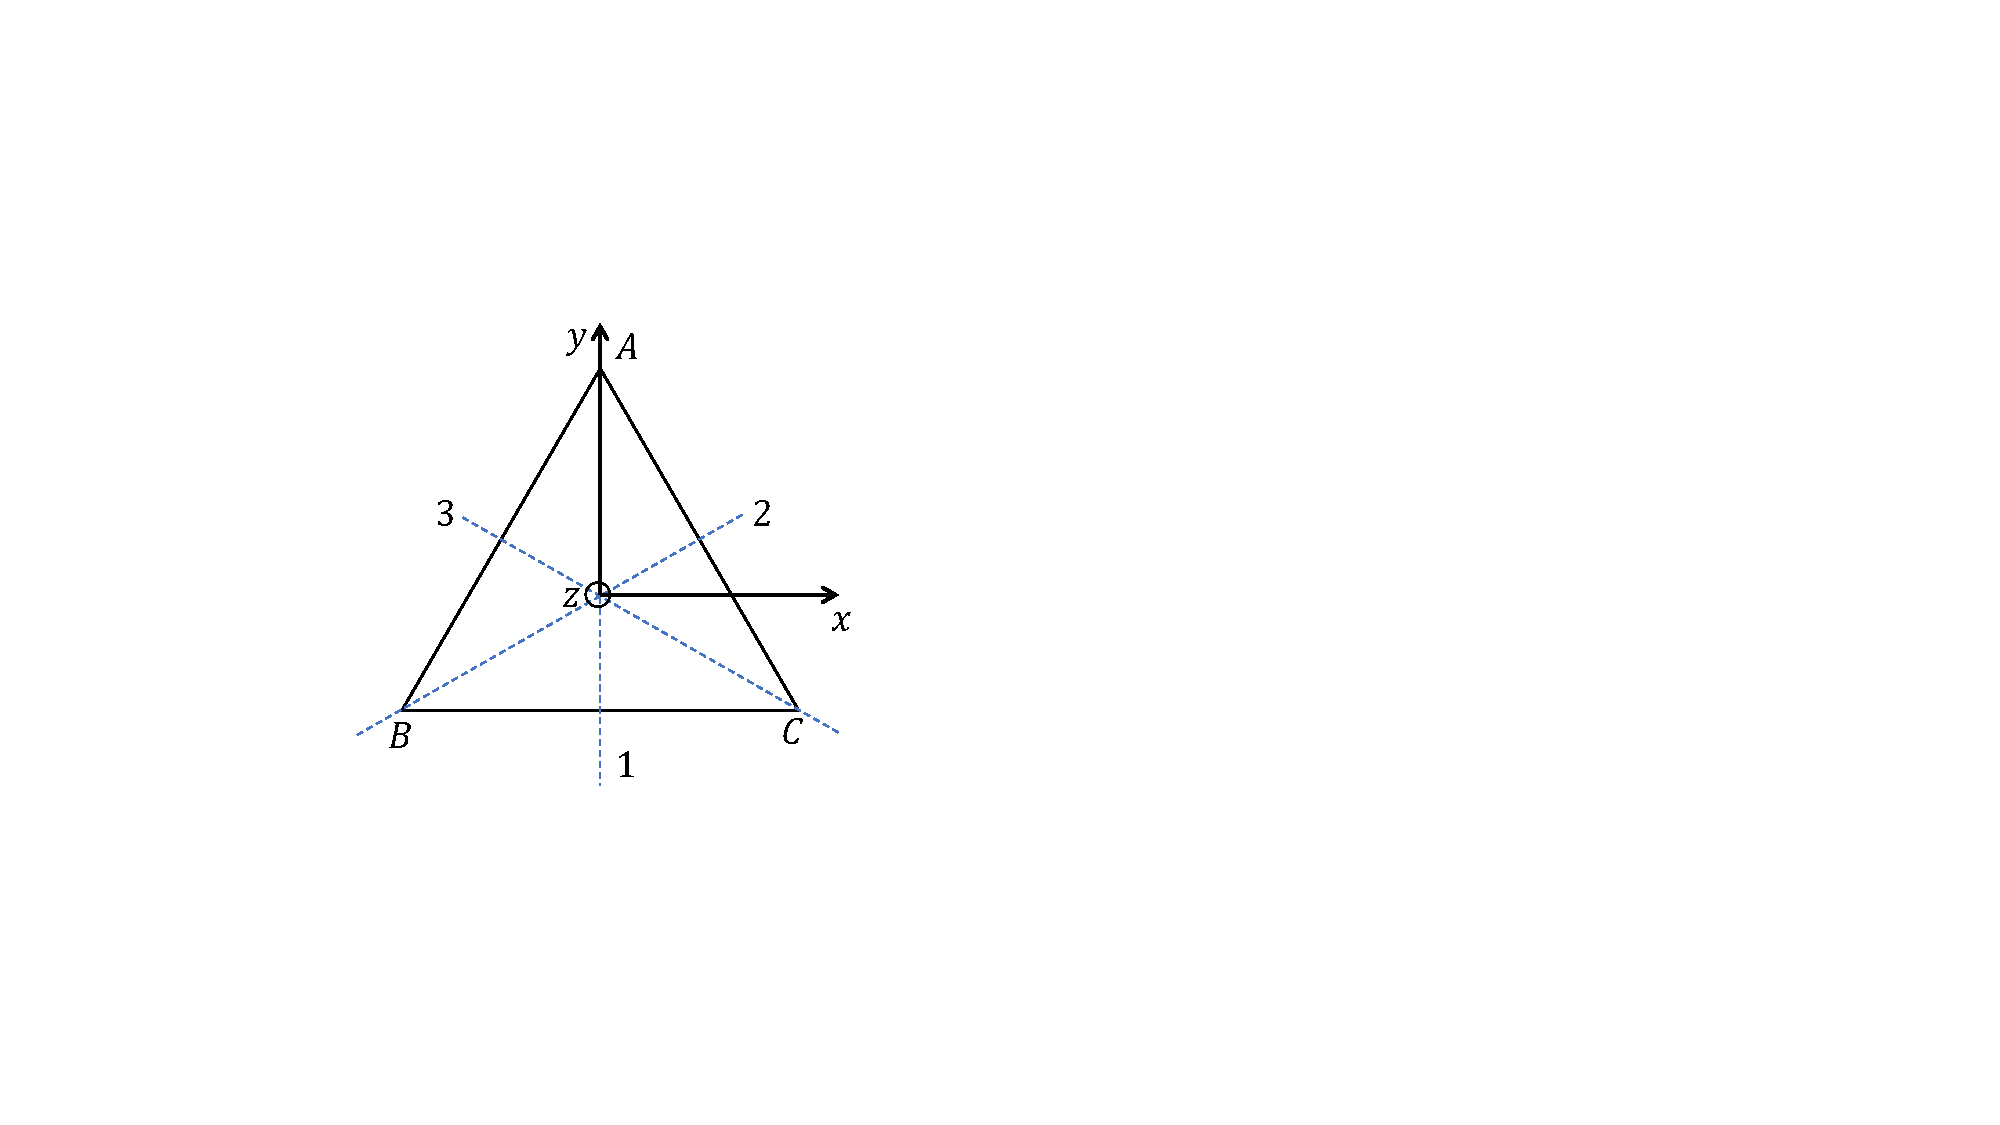
\includegraphics[width=.5\linewidth]{fig/D-1.pdf}}%
		\tablebox{\caption{$D_3$群特征标表}}{%
			\label{tab:D.4}
			\begin{tabular}{c|c|c|c}
				\hline
				& $1\{e\}$ & $2\{d,f\}$ & $3\{a,b,c\} $\\
				\hline$\mathscr{A}^1$ & $1$ & $1$ & $1$ \\
				\hline$\mathscr{A}^2$ & $1$ & $1$ & $-1$ \\
				\hline$\mathscr{A}^3$ & $2$ & $-1$ & $0$ \\
				\hline
		\end{tabular}}
	\end{floatrow}
\end{figure}

我们还是举$D_3$群的例子,这次的任务不是求特征标这些,而是求具体的表示,求群在具体的某个函数空间上的表示。

在举例之前我们要先说明,
$D_3$

有限群最重要的部分我们就讲完了,这个附录最开始的部分我们引用了杨振宁的一句话,看了这些群论定理的证明,你应该能稍微体会到这句话了。

\section{置换群}